\section{Introduction}
This chapter describes the methods used to for derive the first Jet Energy Scale (JES) insitu calibrations for large-R jets using \zjets events, for jets that have been reconstructed using UFO input objects (Section \ref{sec:atlas:jets}). The JES is derived in the region $|\eta|<0.8$, for large-R jets with $152.2\GeV < \pt < 754.6\GeV$ for \zee events and $156.9\GeV<\pt<745.4\GeV$ for the \zmm events. The calibration was derived using the ``InsituBalance'' framework, which is a software package originally created for the MultiJet-Balance calibration \cite{Atlas:largercali}, but was adapted by the author for the Z+jet insitu calibrations.% The workflow of the InsituBalance framework is outline in Figure \ref{fig:insituworkflow}, which is a flowchart that shows each step of the calibration in going from the input samples to the final graphs which are passed on the insitu combination effort. 
%In the insitu combination, the results from all insitu calibration steps are combined to yield the final calibrations used by physics analyses.
%\begin{figure}[t]
%    \centering
%    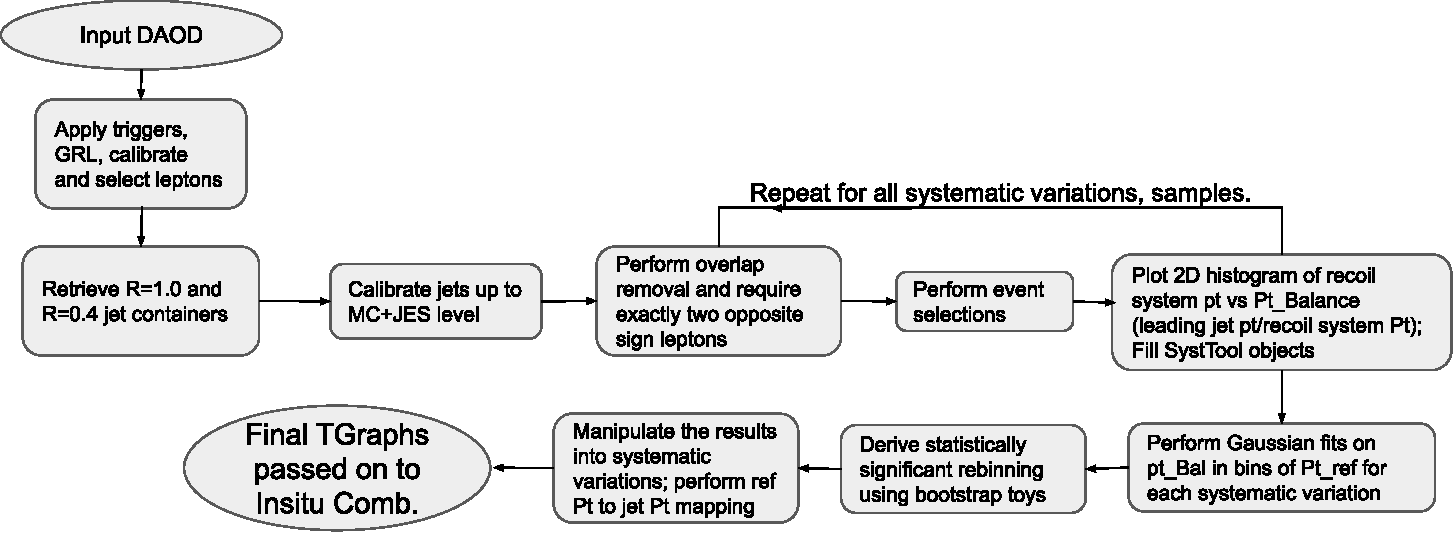
\includegraphics[width=\textwidth]{plots/insitu/workflow.pdf}
%    \caption{Flowchart showing the workflow for the InsituBalance framework used in the deriving the $Z+$jet large-R calibration.\label{fig:insituworkflow}}
%\end{figure}

\section{Jet Calibration\label{sec:jetcal}}

After reconstruction, jets are calibrated so that the average reconstructed jet \pt and mass, $m$, is restored to that of particle-level (also called \textit{truth}) jets. These are simulated jets which have not gone through detector simulation. The correction factors are known as jet energy/mass scale (JES,JMS) factors. The JES+JMS calibration consists of a series of steps outlined in Figure \ref{fig:jetcali}, where the steps are slightly different for small-R and large-R jets.

\begin{figure}[t]
    \centering
    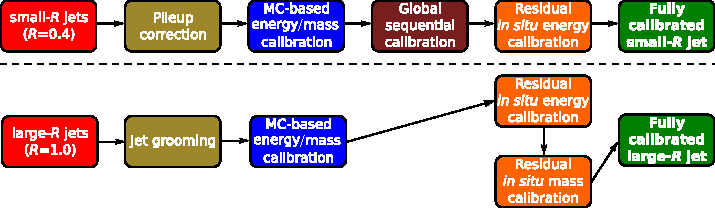
\includegraphics[width=\textwidth]{plots/atlas/calichain.pdf}
    \caption{Jet calibration chain for small-R and large-R jets. Adapted from \cite{Schramm:2017frb}.\label{fig:jetcali}}
\end{figure}

After anti-$k_t$ jet building of the detector-level (also called \textit{reco}) jets - these are simulated jets which have gone through detector simulation - a reference set of truth jets are reconstructed and geometrically matched to the reco jets using a $\Delta R$ matching requirement. Small-R jets then have a pileup correction applied in the first stage of the calibration chain. The purpose of this step is to correct for the contribution to the jet energy due to pileup. The correction consists of two steps: the jet area-based correction and the residual pileup correction. The area-based corrections subtracts the expected contribution from pileup based on the area of the jet and the median \pt density in the event. After this correction there is still a dependence of the difference between the reco jet and truth jet \pt on the pileup activity. A residual correction is therefore implemented, parametrised in the number of PVs ($N_{\text{PV}}$), and $\mu$ which quantify in-time and out-of-time pileup\footnote{in-time pileup refers to $pp$ collisions from the same bunch-crossing as the interaction of interest, whereas out-of-time pileup refers to $pp$ collisions occurring in bunch-crossings just before and after the interaction of interest.} respectively.

Large-R jets do not have a pileup correction applied in the same way as small-R jets. Since the jet volume of large-R jets encloses a larger fraction of the calorimeter than small-R jets, they are significantly more sensitive to pileup. In spite of the fact that large-R jets represent high \pt objects, and pileup is typically low \pt, the angular structure of large-R jets can be affected, limiting the jet substructure performance. For this reason, ``grooming'' algorithms are applied to large-R jets. Grooming algorithms remove jet constituents, and rebuild the jets from the remaining constituents. The ``trimming'' algorithm was prevalent for large-R jets in early Run-2 analyses, where regions of the jet with small relative contributions to the jet \pt are removed. The latest recommendations use variations of the ``Soft-Drop'' algorithm, which is a technique for removing soft and wide-angle radiation from a jet. With the reconstruction of large-R truth jets, the same grooming algorithm is applied as the reco jets.  

In the next step of the calibration chain, the MC-based JES and JMS corrections are derived using dijet events. The \pt and mass responses are defined as $R_{\pt}=\langle\pt^{\text{reco}}/\pt^{\text{true}}\rangle$ and $R_{m}=\langle m^{\text{reco}}/m^{\text{true}}\rangle$, where the averages are determined from Gaussian fits (recently, small-R UFO jets were calibrated using a ``numerical inversion'' technique which uses piecewise polynomials called ``splines'' to fit the response \cite{Atlas:smallrufo}). For the JES calibration, the response fits are performed in bins of jet energy and detector pseudorapidity (pseudorapidity relative to the geometrical center of the ATLAS detector, rather than the hard scatter PV). The JES factor, $c_{\text{JES}}=1/R_{\pt}$ is then smoothed in energy and $\eta_{\text{det}}$. A correction to $\eta$, $\Delta\eta$ is also derived. After $c_{\text{JES}}$ is calculated, a correction to the jet invariant mass is derived\footnote{Corrections to the large-R jet mass in particular are important since the mass is more sensitive than the \pt to soft, wide-angle contributions, calorimeter geometry and topo-cluster merging and splitting. Moreover, the large-R jet mass is a powerful substructure variable used for discriminating between QCD jets and hadronically decaying massive particles.}. Jet mass corrections are derived using the same procedure as the JES, and in bins of $E_{\text{reco}}$, $\eta^\text{det}$, as well as $\log(m_{\text{reco}}/E_{\text{reco}})$. The JMS calibration factor ($c_{\text{JMS}}=1/R_m$) is applied only to the mass of the jet while keeping the energy fixed, and allowing the \pt to vary.  The $\phi$  coordinate is not affected by the calibration. The calibrated kinematic variables are thus given by: 
\begin{equation}
    E_{\text{reco}}=c_{\text{JES}}E_0,\hspace{5pt}m_{\text{reco}}=c_{\text{JES}}c_{\text{JMS}}m_0,\hspace{5pt}\eta_{\text{reco}}=\eta_0+\Delta\eta,\hspace{5pt}\pt^{\text{reco}}=c_{\text{JES}}\frac{\sqrt{E_0^2-c_{\text{JMS}}^2m_0^2}}{\cosh(\eta_0+\Delta\eta)},
\end{equation}
where the quantities with a 0 subscript refer to those prior to any calibration, but after jet grooming (for the large-R case) \cite{Atlas:largercali,Atlas:Schramm}.

For small-R jets, there is an additional step after the MC-based calibration, which is the Global Sequential Calibration (CSC). This step aims to improve the relative \pt resolution given by $\frac{\pt^{\text{JES+JMS}}/\pt^{\text{true}}}{\langle\pt^{\text{JES+JMS}}/\pt^{\text{true}}\rangle}$, where $\pt^{\text{JES+JMS}}$ is the jet transverse momentum after the MC-based calibration. The GSC also corrects for differences in the \pt response for gluon initiated and quark initiated jets. This correction is derived based on global jet observables such as the longitudinal shower structure, and tracking information, and takes the form of a sequence a multiplicative corrections. Recently a neural network approach (Global Neural Network Calibration) has been explored which is an alternative to this sequential correction and allows for correlated global observables to be used in deriving the calibration \cite{Atlas:smallrnewtechniques}.

The final calibration stage is the \textit{in situ} calibration. Differences in the jet response can arise between data and simulation due to imperfect detector modelling, pileup, particle-detector interactions, the UE, and jet formation. The in situ correction factor is defined as the double ratio of the response in data divided by the response in MC:
\begin{equation}
    c=\frac{\mathcal{R}^{\text{data}}_{\text{in situ}}}{\mathcal{R}^{\text{MC}}_{\text{in situ}}},
\end{equation}
where the response is defined as:
\begin{equation}
    \mathcal{R}_{\text{in situ}} = \Bigg\langle\frac{\pt^{\text{jet}}}{\pt^{\text{ref}}}\Bigg\rangle,
\end{equation}
and $\pt^{\text{ref}}$ is defined as the \pt of a well-measured reference object, and $\pt^{\text{jet}}$ is the transverse momentum of the jet being calibrated. $\mathcal{R}_{\text{in situ}}$ is transformed from a function of $\pt^{\text{ref}}$ to a function of jet transverse momentum through a process of numerical inversion (see Section \ref{sec:insitu}) prior to the double ratio $c$ calculation. The response $\mathcal{R}_{\text{in situ}}$ is sensitive to secondary effects such as out-of-cone radiation, where jets from QCD radiation are not captured by the jet cone. The expectation is therefore that $\mathcal{R}_{\text{in situ}}$ is skewed below 1, and these effects are partially mitigated through the event selection. The double ratio $c$, however, is robust to such effects, so long as they are not mismodelled in simulation. 

There are three stages of the insitu calibration which are performed sequentially. First, the inter-$\eta$ calibration uses dijet events to correct the energy scale of forward jets ($0.8 < |\eta_{\text{det}}| < 4.5$) to that of central jets ($|\eta_{\text{det}}|<0.8$). The reason for deriving this correction is that the in situ calibrations that follow are derived solely in the central region as forward jets have increased response variations due to the more complicated detector structure in the forward regions. The $\eta$-inter calibration requires two back-to-back jets in the transverse plane from different $\eta_{\text{det}}$ regions. All insitu calibration steps exploit the momentum balance of the system. In the case of the $\eta$-inter calibration, the two jets are required to have equal and opposite \pt to satisfy the momentum balance. A quantity called the momentum asymmetry is constructed, which is the difference of the jet transverse momenta divided by the average jet \pt, and quantifies the response difference between the two detector regions. For a given pair of $\eta_{\text{det}}$, the asymmetry can be used to define the calibration factors.

The next step of the calibration chain exploits the \pt balance in $\gamma/Z(\rightarrow ee/\mu\mu)$+jet events. Electrons and photons are accurately calibrated as described in Section \ref{sec:egamma}, and the muons are calibrated using $Z\rightarrow\mu\mu$, $J/\Psi\rightarrow\mu\mu$ and $\Upsilon\rightarrow\mu\mu$ events. These methods benefit from the accurate knowledge of the energy scale and resolution of leptons and photons. These in situ calibrations are called the direct-balance (DB) calibrations. The DB response is:
\begin{equation}
    \mathcal{R}_{\text{DB}}=\langle\frac{\pt^{\text{j1}}}{\pt^{\text{ref}}}\rangle,\hspace{5pt}\pt^{\text{ref}}=\pt^{Z\gamma}|\cos(\Delta\phi)|,
\end{equation}
where $\pt^{\text{j1}}$ is the \pt of the leading jet, and $\Delta\phi$ is the azimuthal separation between the photon or the reconstructed $Z$. The reason for the $|\cos\Delta\phi|$ factor is to reduce the effect of ``out-of-cone'' (OOC) radiation, which is additional QCD radiation from the jet which is not captured in the jet cone during jet building. The reference object is colour neutral, hence there is more QCD radiation in the jet hemisphere resulting in a bias which takes the response below unity. This $|\cos\Delta\phi|$ factor reduces the effect of this bias by balancing the momentum of the reference object onto the jet axis in the transverse plane. 

Events are selected by requiring low \pt jet veto, and a minimum requirement on the $\Delta\phi$ between the leading jet and the reference system. Independent calibration factors are derived for $Z(\rightarrow ee)$+jet, $Z(\rightarrow \mu\mu)$+jet and $Z\gamma$+jet DB. The $Z$+jet calibration is limited to the statistically significant \pt range of $Z$ boson production, and is therefore only relevant at low and medium \pt in the range of around $17 < \pt < 800\GeV$. The complementary $\gamma$+jet measurements which are limited by small numbers of events at high \pt and by dijet contamination, are relevant at around $30<\pt<2000\GeV$ with a limited precision at $\pt<100\GeV$.

For the calibration of small-R jets, an additional insitu calibration called the Missing Momentum Fraction (MPF) method is also used to complement the DB calibrations. The MPF method measures the \pt balance between the reference object and the full hadronic recoil (i.e. including any QCD OOC radiation). This method is very robust against pileup and the UE, and covers a similar kinematic range to $\gamma$+jet DB. In the final stage of the insitu calibration, a \pt balance method using multijet events is implemented to extend the kinematic range of the calibration to larger transverse momenta than what could be achieved by $\gamma$+jet. Recent developments in the insitu calibration have allowed for a precision of the correction factor at level of $1\%$. Additionally, recent developments have allowed for measurements of the JES for b-tagged jets at the level of $1\%$ using $\gamma$+jet direct balance. These measurements have the potential to improve the precision of analyses which are very sensitive to the b-jet JES such as $H\rightarrow b\bar{b}$ and top mass measurements \cite{Atlas:smallrnewtechniques,Atlas:largercali,Atlas:smallrcali}.

For the case of large-R jets, an in situ calibration for the JMS is also calculated. Two independent methods are used to derive these corrections. The $R_{\text{trk}}$ method uses calorimeter-to-tracker response ratios. This method was used for calibrating large-R LCTopo jets for Run-2 analyses, where the fact that tracker and calorimeter provide independent measurements is exploited in order to validate the modelling of large-R jet properties. The forward folding method uses a high purity, high \pt large-R jet sample from $t\bar{t}$ events, where one of the top quark decays hadronically ($t\rightarrow b+W(\rightarrow\text{jets})$), and the other decays via a leptonically decaying W ($t\rightarrow b+W(\rightarrow l\nu)$). The response is obtained from fits to the top and W mass peaks in the invariant mass distribution of the large-R jet of the hadronically decaying top candidate. The W mass peak is present when a large-R b-jet veto is applied, and the top mass peak is present when the large-R jet is b-tagged. Two independent methods for calculating the large-R jet mass are implemented. These are the calorimeter jet mass, $m^{\text{calo}}$, and the track-assisted jet mass ($m^{\text{TA}}$). For a large-R calorimeter jet $J$ with topo-cluster constituents $i$ with energy $E_i$ and momentum $\mathbf{p}_i$, the calorimeter-based jet mass is defined as:
\begin{equation}
    m^{\text{calo}}=\sqrt{(\sum_{i\in J}E_i)^2-(\sum_{i\in J}\mathbf{p}_i)^2},
\end{equation}
and the track-assisted jet mass is defined as:
\begin{equation}
    m^{\text{TA}}=\frac{\pt^\text{calo}}{\pt^\text{track}}\times m^{\text{track}},
\end{equation}
where the track invariant mass, $m_{\text{trk}}$, is assumed to be the pion mass. The values for the response in data and MC are extracted simultaneously in a fit known as \textit{forward folding} \cite{Atlas:largercali}.

%\clearpage
\section{Data and MC samples\label{sec:insitu:dataandmcsamples}}
 Proton-proton collision data at a centre-of-mass energy of $\sqrt{s}=13\TeV$ are using in the in-situ calibration. The data are required to pass unprescaled dielectron or dimuon triggers depending on whether the $Z$-boson decays to electrons or muons, respectively. These triggers are shown in Table \ref{tab:Insitu:trigger}, and depend on the year the data were recorded.
\begin{table}[t]
\centering
\begin{tabular}{|c||c|c|c|}
\hline
& \textbf{Year} & \textbf{Level1} & \textbf{HLT} \\ \hline \hline
\multirow{7}{*}{\textbf{Dielectron trigger}} 
%& \multirow{2}{*}{2015} & xyz \\ && centred on $\et=12\GeV$ & \multirow{2}{*}{N/A} \\
& \multirow{2}{*}{2015} & $\et>10\GeV$(*); & $\et>12\GeV$; \\ & & Hadronic activity veto & loose ID \\ \cline{2-4} & \multirow{2}{*}{2016} & $\et>13\GeV$(*); & $\et>15\GeV$; \\ & & Hadronic activity veto & vloose ID, $d0$ unused \\ \cline{2-4} & \multirow{3}{*}{2017/2018} & $\et>15\GeV$(*); & \multirow{2}{*}{$\et>17\GeV$;} \\ & & Hadronic activity veto; & \multirow{2}{*}{vloose ID, $d0$ unused} \\ & & Isolated & \\
\hline \hline
\multirow{4}{*}{\textbf{Dimuon trigger}} 
%& \multirow{2}{*}{2015} & xyz \\ && centred on $\et=12\GeV$ & \multirow{2}{*}{N/A} \\
& \multirow{2}{*}{2015} & \multirow{2}{*}{$\et>10\GeV$} & \multirow{2}{*}{ $\et>10\GeV$} \\ &&&\\ \cline{2-4} & \multirow{2}{*}{2016/2017/2018} & \multirow{2}{*}{$\et>10\GeV$} & \multirow{2}{*}{$\et>14\GeV$} \\ & & & \\
\hline
\end{tabular}
\caption{An $\eta$-dependence of the L1 trigger threshold is denoted by (*).\label{tab:Insitu:trigger}}
\end{table}    
 The dataset corresponds to an integrated luminosity of 139\invfb \cite{LUMI}. The data are required to pass data-quality criteria to ensure the data were taken during periods where the detector subsystems were fully functioning. This is achieved via ``GoodRunsLists (GRLs)'', which are provided by the ATLAS Data Quality group.

The nominal sample of \zjet events is generated using \POWHEGBOX v1 \cite{Insitu:powheg1,Insitu:powheg2,Insitu:powheg3}, with NLO matrix-element (ME) accuracy in perturbative QCD for inclusive $Z$ production. The CT10 PDF set is used in the ME calculation \cite{Insitu:ct10}. The parton-level final state is interfaced with \PYTHIA (v8.186) \cite{Insitu:pythia} for generating the parton shower (PS), hadronisation, and multi parton interactions (MPI), utilising the \AZNLO tuned parameter set \cite{Insitu:aznlo}. The \PHOTOSpp program \cite{Insitu:photos} is used for the modelling of QED emissions from electroweak vertices and charged leptons. EvtGen 1.2.0 \cite{Insitu:evtgen} is used for the properties of $b$- and $c$-hadron decays.

For evaluating the systematic uncertainty due to MC generator choice, a second \zjets sample is generated using \SHERPA{2.2.1} \cite{Insitu:sherpa,Insitu:sherpa22} and is subdivided (sliced) into discrete regions of $\text{max}(H_\text{T},p_{\text{T}}^V)$, with boundaries at [0,70,140,280,500,1000,6500]\GeV, where $H_\text{T}$ is defined as the scalar sum of all partonic jet transverse momenta, and $p_{\text{T}}^V$ is the mass of the dilepton system. NLO-accurate matrix elements for up to two jets, and LO-accurate matrix elements for up to 4 jets are calculated with \COMIX \cite{Insitu:comix}. The $b$- and $c$-quarks are treated as massless at the ME calculation, and massive in the parton shower. The parton showering is conducted by \CSShower \cite{Insitu:csshower}, which is based on Catani-Seymour dipole factorisation \cite{Insitu:csalgorithm}. Virtual QCD corrections to the ME are derived with \OPENLOOPS \cite{Insitu:openloops}. The NLO matrix elements for any given jet multiplicity is matched to parton shower, and different jet multiplicities are then merged according to the CKKW matching procedure \cite{Insitu:ckkw1,Insitu:ckkw2} and extended to NLO accuracy using the \MEPSatNLO prescription \cite{Insitu:meps}. The \NNPDF PDF set \cite{Insitu:nnpdf} is used with dedicated parton shower tuning developed by the \SHERPA authors. The invariant mass of the dilepton system is required to be at least $40\GeV$ \cite{Insitu:zjetmc}. The MC event simulations are interfaced with the \GEANT toolkit \cite{GEANT4} for detailed modelling of the ATLAS detector response \cite{Insitu:atlassim}. %These simulations are compared to a data set of $pp$ collisions delivered by the LHC at a centre-of-mass energy of $\sqrt{s}=13\TeV$ during the 2015-2018 period. The data are required to pass unprescaled dielectron or dimuon triggers depending on whether the \zeejet or \zmmjet calibration is performed. These triggers are shown in Table \ref{tab:Insitu:trigger}.
%\begin{table}[ht]
%\centering
%\begin{tabular}{|c||c|c|c|}
%\hline
%& \textbf{Year} & \textbf{Level1} & \textbf{HLT} \\ \hline \hline
%\multirow{7}{*}{\textbf{Dielectron trigger}} 
%& \multirow{2}{*}{2015} & xyz \\ && centred on $\et=12\GeV$ & \multirow{2}{*}{N/A} \\
%& \multirow{2}{*}{2015} & $\et>10\GeV$(*); & $\et>12\GeV$; \\ & & Hadronic activity veto & loose ID \\ \cline{2-4} & \multirow{2}{*}{2016} & $\et>13\GeV$(*); & $\et>15\GeV$; \\ & & Hadronic activity veto & vloose ID, $d0$ unused \\ \cline{2-4} & \multirow{3}{*}{2017/2018} & $\et>15\GeV$(*); & \multirow{2}{*}{$\et>17\GeV$;} \\ & & Hadronic activity veto; & \multirow{2}{*}{vloose ID, $d0$ unused} \\ & & Isolated & \\
%\hline \hline
%\multirow{4}{*}{\textbf{Dimuon trigger}} 
%& \multirow{2}{*}{2015} & xyz \\ && centred on $\et=12\GeV$ & \multirow{2}{*}{N/A} \\
%& \multirow{2}{*}{2015} & \multirow{2}{*}{$\et>10\GeV$} & \multirow{2}{*}{ $\et>10\GeV$} \\ &&&\\ \cline{2-4} & \multirow{2}{*}{2016/2017/2018} & \multirow{2}{*}{$\et>10\GeV$} & \multirow{2}{*}{$\et>14\GeV$} \\ & & & \\
%\hline
%\end{tabular}
%\caption{An $\eta$-dependence of the L1 trigger threshold is denoted by (*).\label{tab:Insitu:trigger}}
%\end{table}    
%The dataset corresponds to an integrated luminosity of 139 \invfb \cite{LUMI}. The data are required to pass data-quality criteria. This is to ensure that the data taken during periods where the detector subsystems were not fully functioning; where there where large amount of detector noise; or where there were read-out issues are discarded. This is achieved via GoodRunsLists (GRLs):
%\begin{itemize}
%    \item 
%    \begin{verbatim} GoodRunsLists/data15_13TeV/20170619/data15_13TeV.periodAllYear_DetStatus-v89-pro21-02_Unknown_PHYS_StandardGRL_All_Good_25ns.xml
%    \end{verbatim}
%    \item 
%    \begin{verbatim} GoodRunsLists/data16_13TeV/20180129/data16_13TeV.periodAllYear_DetStatus-v89-pro21-01_DQDefects-00-02-04_PHYS_StandardGRL_All_Good_25ns.xml 
%    \end{verbatim}
%    \item 
%    \begin{verbatim} GoodRunsLists/data17_13TeV/20180619/data17_13TeV.periodAllYear_DetStatus-v99-pro22-01_Unknown_PHYS_StandardGRL_All_Good_25ns_Triggerno17e33prim.xml
%    \end{verbatim}
%    \item 
%    \begin{verbatim} GoodRunsLists/data18_13TeV/20190318/data18_13TeV.periodAllYear_DetStatus-v102-pro22-04_Unknown_PHYS_StandardGRL_All_Good_25ns_Triggerno17e33prim.xml
%    \end{verbatim}
%\end{itemize}
%
%\begin{VerbItem}
%    GoodRunsLists/data15_13TeV/20170619/data15_13TeV.periodAllYear_DetStatus -v89-pro21-02_Unknown_PHYS_StandardGRL_All_Good_25ns.xml
%    GoodRunsLists/data16_13TeV/20180129/data16_13TeV.periodAllYear_DetStatus -v89-pro21-01_DQDefects-00-02-04_PHYS_StandardGRL_All_Good_25ns.xml 
%    GoodRunsLists/data17_13TeV/20180619/data17_13TeV.periodAllYear_DetStatus -v99-pro22-01_Unknown_PHYS_StandardGRL_All_Good_25ns_Triggerno17e33prim.xml
%    GoodRunsLists/data18_13TeV/20190318/data18_13TeV.periodAllYear_DetStatus -v102-pro22-04_Unknown_PHYS_StandardGRL_All_Good_25ns_Triggerno17e33prim.xml
%\end{VerbItem}
%
%JETM3 DAOD datasets are used which are designed specifically for the \zjets insitu calibration as well determination of the combined performance MET systematics. These derivations contain the relevant jets described in Section \ref{sec:jetdef}, and are skimmed by requiring two single or dilepton triggers, and two leptons with $\pt>\sim20\GeV$. 
%TODO: Write about derivations before the reconstruction section.
% Derived xAODs (DAODs) in the JETM3 format are used 
%
%Trigger requirements, ATLAS standard quality criteria, data from periods where detector subsystems not fully functional is discarded, or where there is large detector noise, or read-out problems - good run lists. Int lumi of 139\invfb.  of ATLAS detector data collected during run2 in the 2015-2018 data-taking period at a centre-of-mass energy of $\sqrt{s}=13\TeV$.
%\clearpage
\section{Jet definitions \label{sec:jetdef}}
The large-R jets, which are the subject of the insitu calibration described in this chapter, are built from UFO jet input objects \cite{Atlas:UFO} using the anti-$k_t$ algorithm \cite{Insitu:antikt} with radius parameter $R=1.0$. Constituent-level pile-up mitigation is applied using the Constituent Subtraction (CS) \cite{Insitu:cs} and SoftKiller (CS) \cite{Insitu:sk} algorithms. To remove soft contributions from the reconstructed jet, the Soft-Drop (SD) grooming algorithm \cite{Insitu:softdrop} is implemented. Additionally, fully calibrated small-R jets \cite{Atlas:PFlow2,Insitu:smallrcali} are used for \pt balancing and jet veto purposes. These jets are built from Particle Flow (PFlow) \cite{Atlas:PFlow} input objects using the anti-$k_t$ algorithm with radius parameter $R=0.4$. An overview of the definitions of the different jet objects is shown in Table \ref{tab:jetdefs}. The specific implementation of the jet clustering algorithm is taken from the \FASTJET package \cite{Insitu:fastjet1,Insitu:fastjet2}.

Large-R jets are calibrated in both data and simulation up the MC-based JES and JMS (MC JES+JMS) calibration scale \cite{Atlas:largercali}. Small-R jets are fully calibrated in both data and simulation, as described in Section \ref{sec:jetcal}.
%TODO: Describe smearing and describe CS+SK and Soft drop...
\begin{table}[t]
    \centering
    \begin{tabular}{|c||c|c|c|}
    \hline
    & \textbf{Algorithm} & $R$ & \textbf{Settings} \\ \hline \hline
    \multirow{4}{*}{\textbf{Jet input objects}} 
    & \multirow{2}{*}{Particle-Flow}          & \multirow{2}{*}{0.4} & \multirow{2}{*}{N/A} \\
                & & &        \\ \cline{2-4}
    & \multirow{2}{*}{Unified Flow Objects}    & \multirow{2}{*}{1.0} & \multirow{2}{*}{N/A} \\
                            & & &        \\
    \hline \hline
    \multirow{5}{*}{\textbf{Pile-up mitigation algorithms}} & \multirow{3}{*}{Constituent Subtraction} & \multirow{3}{*}{1.0}
                             & $A_g = 0.01$ \\
    &                        & & $\DeltaR_\text{max} = 0.25$ \\
    &                        & & $\alpha = 0$ \\ \cline{2-4}
    & \multirow{2}{*}{SoftKiller}             & \multirow{2}{*}{1.0}
                             & \multirow{2}{*}{$\ell = 0.6$} \\ &&& \\ 
    \hline \hline
    \multirow{2}{*}{\textbf{Jet grooming algorithms}}
    & \multirow{2}{*}{Soft-Drop} & \multirow{2}{*}{1.0}
                             & $\zcut$ = 0.1     \\
    &                      & & $\beta$ = 1    \\ \cline{2-4}
    \hline %inserts single line
    \end{tabular}
    \caption{Summary of the jet input object algorithms used for small-R ($R=0.4$) and large-R ($R=1.0$) jets, in addition to the specific pile-up mitigation and grooming algorithms used for the large-R jets. Since different versions of the pile-up and grooming algorithms exist, the exact parameters used relevant to these algorithms is shown in the last column. See \cite{Insitu:cs,Insitu:sk,Insitu:softdrop} for further details on the parameters.\label{tab:jetdefs}.} %Summary of pile-up mitigation algorithms, jet inputs, and grooming algorithms, the relevant parameters for each algorithm. \label{tab:jetdefs}}
    \end{table}    

%\clearpage
\section{Object Selections\label{sec:insitu:largerobj}}
\subsection{Electrons}
Electrons are reconstructed from ID tracks and calorimeter information as described in section \ref{sec:egamma}. Electrons are calibrated using the ``EgammaCalibrationAndSmearingTool'' with the ESModel ``es2018\tu R21\tu v0'' configuration using the decorrelation model setting ``1NP\tu v1'', which results in one non-zero scale and resolution systematic variation. Electrons are required to satisfy \textit{Loose} ID, and \textit{FCLoose} isolation requirements\footnote{``FC'' refers to ``FixedCut'', i.e. that a cut is put on the isolation variables themselves, rather than using cut maps to achieve a target selection efficiency.}, and are reconstructed within $|\eta|<2.47$, excluding the gap between the barrel and endcap EM calorimeters (1.36 < $|\eta|<1.52$). Electrons are required to satisfy $\pt>20\GeV$. Electrons are constrained to originate from the primary hard-scatter vertex through the requirements $|d_0|/|{\sigma_{d_0}}|<5$ and $|z_0\sin\theta|<0.5\mm$, where the impact parameters are defined in Section \ref{sec:tracking}.
\subsection{Muons}
Muons are reconstructed from MS tracks matched to ID tracks as described in Section \ref{sec:muon}. Muons are calibrated using the ``MuonCalibrationAndSmearingTool'' and the ``correctData\tu ID\\MS'' scheme which gives muon track resolution and momentum scale systematic variations on the seperate ID and MS components of the combined (CB) muon.  Muons are required to satisfy \textit{Loose} ID, and \textit{FCLoose} isolation requirements, and must be reconstructed within $|\eta|<2.4$ with $\pt>20\GeV$. Muons are constrained to originate from the primary hard-scatter vertex through the requirements $|d_0|/|{\sigma_{d_0}}|<3$ and $|z_0\sin\theta|<0.5\mm$, where the impact parameters are defined in Section \ref{sec:tracking}. The $\eta$ cut, ID quality, and track selections are performed by the ``MuonSelectionTool'', which also facilitaties vetoing events containing mis-reconstructed muons, as these objects tend to have significantly worse momentum resolution. Muons consistent with cosmic ray backgrounds are removed.
\subsection{Jets}
As described in Section \ref{sec:jetcal}, the \zjets insitu calibration is designed to provide residual corrections to jets measured in the central detector region. Therefore, large-R jets are selected to be in the region $|\eta|<0.8$ and with $\pt>100\GeV$. Small-R jets are selected with $\pt>10\GeV$ and $|\eta|<4.5$ and are required to be $\Delta R>1.4$ from the leading large-R jet, to ensure no overlap. Small-R jets with $\pt<60\GeV$ and $|\eta|<2.4$ are required to satisfy the \textit{Tight} Jet Vertex Tagger (JVT) \cite{Insitu:JVT} working point in order to reject additional jets originating from pileup. The \textit{Medium} JVT working point is used as a systematic variation to assess the impact of the JVT selection on the calibration. % Small-R jets used to veto events with large QCD radiation are required to be separated from the the large-R jet where the response is being measured (J1).  
% TODO: Describe JVT
% TODO: Update isolation variables table to be consistent with the twiki page here: https://twiki.cern.ch/twiki/bin/view/AtlasProtected/IsolationSelectionTool#Leptons 
% FixedCutLoose 	electrons 	Cut: topoetcone20/pT < 0.2 	Cut: ptvarcone20/pT < 0.15 

%  1NP_v1: very simplified model. This is suggested for analyses which are not sensitive to the energy scale or resolution and that do not use categories in eta. All the physical effects are summed in quadrature and considered fully correlated in eta. Usually this approach give pessimistic (larger) systematics. Using this scheme it should be checked that in the fit the NPs relative to the calibration systematics are neither pulled nor over-constrained. If this happens it could mean that the analysis is sensitive to the calibration and its decorrelation and so a more detailed model is needed. FROM: https://twiki.cern.ch/twiki/bin/view/AtlasProtected/ElectronPhotonFourMomentumCorrection#Recommendation_for_run_2_data_in
\subsection{Overlap Removal}\label{sec:insitu:or}
To prevent detector signals from one object being used in the reconstruction of a different object, an object overlap removal procedure is applied according to the ATLAS standard overlap removal tool \cite{ORTool} in the following order:
\begin{itemize}
    \item If two electrons share the same track in the ID, the electron with the lowest \pt is rejected.
    \item Calorimeter muons are rejected against electrons if they share the same track in the ID.
    \item Electrons are rejected against muons if they share the same track in the ID.
    \item Small-R jets are rejected against electrons if $\Delta R<0.2$.
    \item Electrons are rejected against small-R jets if $\Delta R<0.4$.
    \item Small-R jets are rejected against muons if there are $<3$ tracks and either the jet and the muon are ghost-associated\footnote{With ``ghost-association'' particles can be associated to jets by treated them as particles with negligible \pt and clustering them within the jet \cite{Insitu:ghostassociation}.} or $\Delta R<0.2$. 
    \item Muons are rejected against small-R jets if $\Delta R<0.4$.
    \item Large-R jets are rejected against electrons if $\Delta R < 1.0$.
\end{itemize}

%\clearpage
\section{Event Selection}
Event selection criteria are applied such that the analysis is performed in a region that is populated by event topologies in which the reconstructed $Z$-boson's momentum is balanced by the momentum of the large-R jet (a so-called 2$\rightarrow$2 topology). Furthermore, to ensure the leptons are consistent with a Z-boson decay, lepton pairs are required to have the same flavour and opposite charge. The invariant mass of the dilepton system is required to be consistent with the invariant mass of the Z-boson, i.e. $66\GeV<m_{ll}<116\GeV$. The $2\rightarrow2$ topology selection is enforced by a veto on events in which (i) there is a small-R jet that carries a significant amount of the total jet momentum, and (ii) the large-R jet and the dilepton system are separated by $\Delta\phi(Z,J_1)\approx\pi$. The event selections and their variations for evaluating systematic uncertainties are listed in Table \ref{tab:evsel_insitu}. 

\begin{table}[t]
    \centering
    \resizebox{\textwidth}{!}{%
    \begin{tabular}{lccc}
        \hline
        Variable & Nominal Selection & Up Variation & Down Variation \\ \hline
        $\pt^{\mathrm{j_1}} $ & $<\max(0.1\,\ptref,15~\GeV)$ & $<\max(0.15\,\ptref,20~\GeV)$ & $<\max(0.05\,\ptref,10~\GeV)$ \\
        $\Delta\phi(Z,\mathrm{J_1})$ & $>2.8$ & $>2.9$ & $>2.7$ \\
        $m_{ll}$ & $66\GeV<m_{ll}<116\GeV$ & --- & --- \\ 
        Lepton charge & Opposite charge pairs & --- & --- \\ \hline
        %Small-$R$ jet JVT  & Tight & --- & Medium \\
    \end{tabular}}
    \caption{Event selection criteria and corresponding systematic variations. The large-R jet with the highest \pt (hardest) is given the label J1. The hardest small-R jet is given the label j1 (not capitalised).\label{tab:evsel_insitu}}
\end{table}
%TODO change pt_ref to pt^ref. All other pt variables should have superscripts as well.
%\clearpage
\section{Nominal Response Calculation}
Measurements of $R_{\text{DB}}$ are carried out separately in the electron and muon channels. These measurements are later combined in the insitu combination effort to provide a single insitu correction. $R_{\text{DB}}$ is measured using a 2D histogram of \ptref and $\ptbal\equiv\frac{\ptJ}{\ptref}$ for every event passing the selection criteria. The binning of \ptref is chosen to be [150, 175, 200, 225, 250, 300, 350, 400, 600, 800] \GeV to match the previous calibration effort for EMTopo large-R jets \cite{Atlas:largercali}. The \ptbal variable has a fine binning to facilitate a Gaussian fit of the response curves. The 2D histogram is shown for \zee events for the response calculation in data in Figure \ref{fig:insitu:2dhistzeedata}.
\begin{figure}[t]
    \centering
    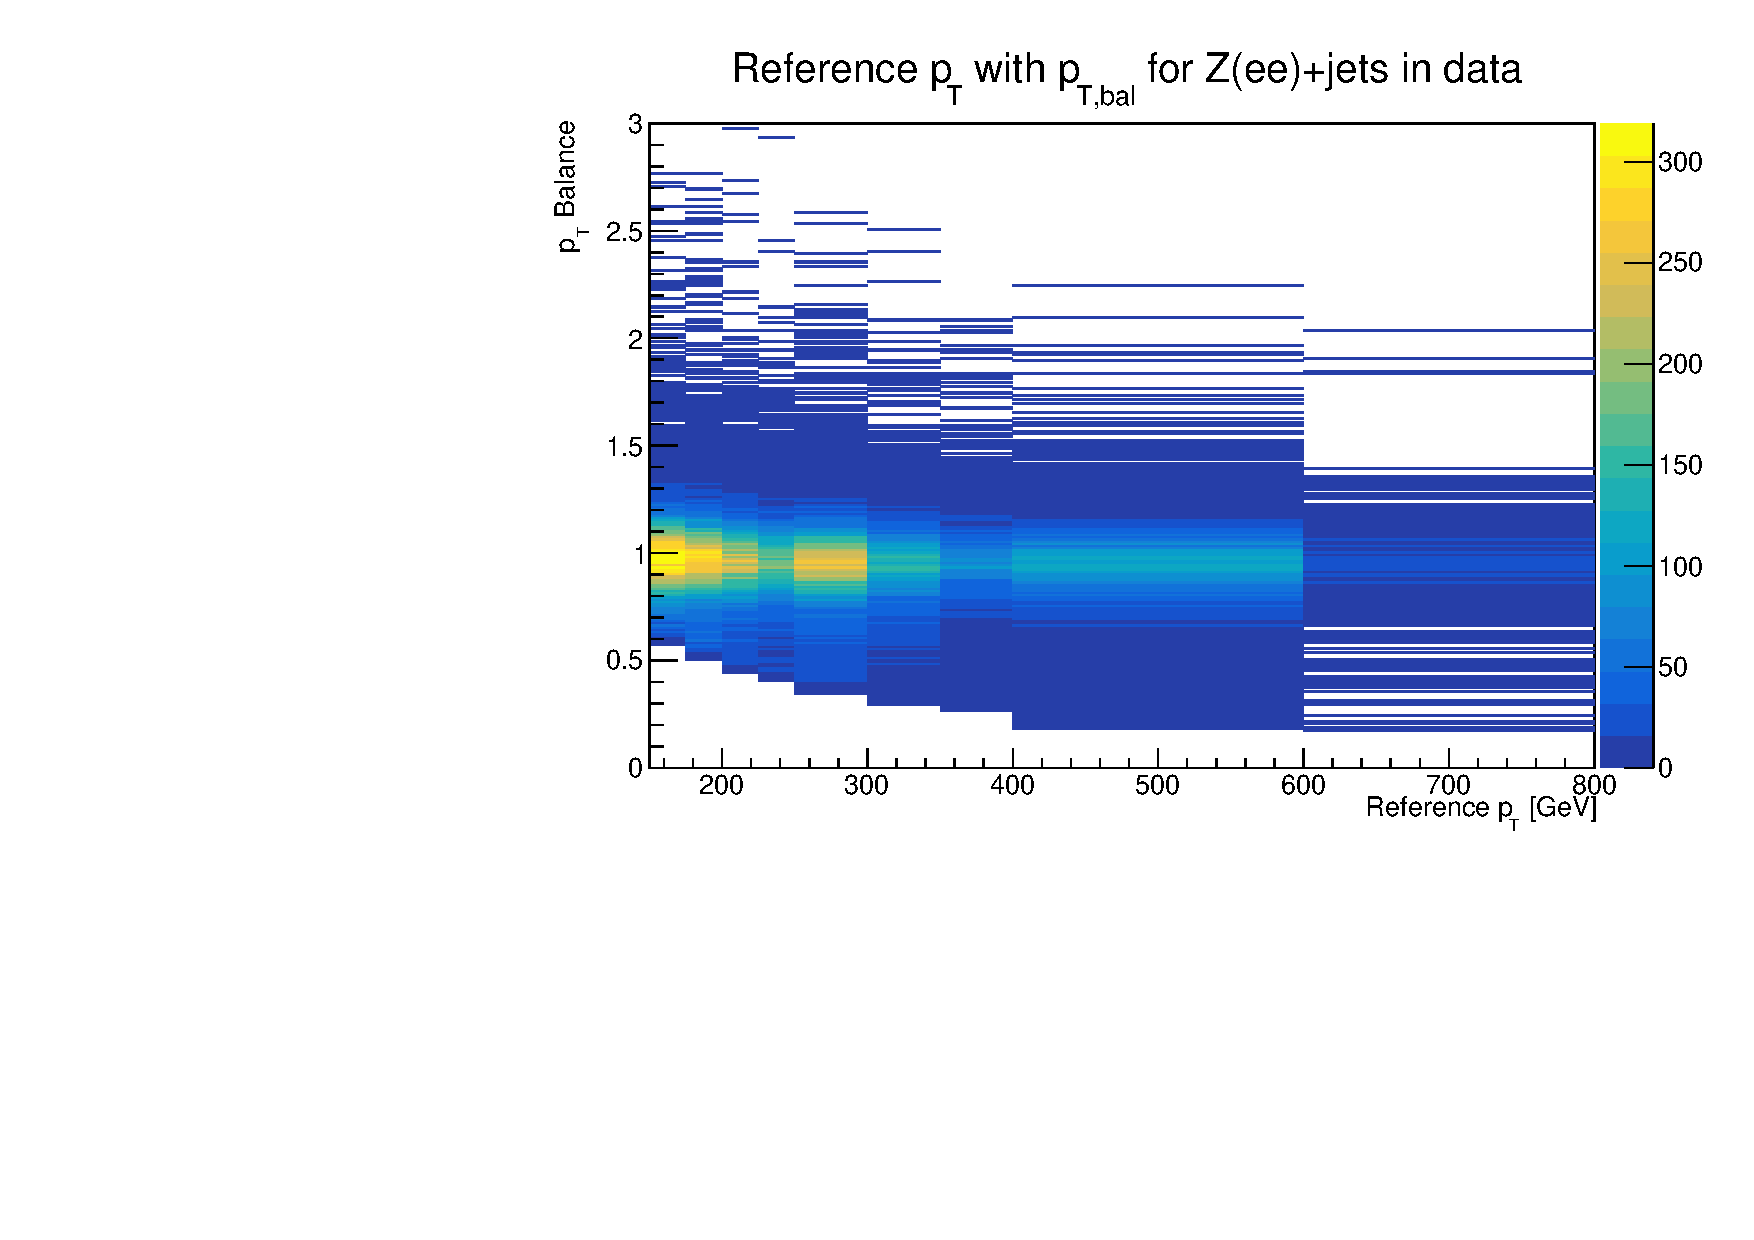
\includegraphics[width=0.8\textwidth]{plots/insitu/Response2D_Data_Zee.pdf}
    \caption{\ptref with \ptbal for \zee events in data. The response distributions in bins of \ptref are y-axis slices of this 2D histogram.\label{fig:insitu:2dhistzeedata}}
\end{figure}

The 2D histogram is sliced in bins of \ptref, and the average response \rdb is determined from the mean of a Gaussian fit. The error on the mean is used to quantify the statistical uncertainty on \ptbal. %%%FROM HERE%%% 

Before performing the fit, each \ptref distribution is uniformly re-binned in accordance to Scott's normal reference rule \cite{Insitu:scottsrule}, which states that the bin width should be as close as possible to $\frac{3.5\sigma_{\text{hist}}}{\sqrt[3]{N}}$ ($\sigma_{\text{hist}}$ is the standard deviation of the histogram and $N$ is the number of events). After re-binning, a Gaussian distribution is fit using a minimum log-likelihood method, where the likelihood is built assuming a Poisson probability density function for each bin \cite{Insitu:likelihoodfit}. This fit is performed over the range $x_{\text{max}}\pm\frac{x_{\text{max}}}{8}$, where $x_{\text{max}}$ is the $x$ value corresponding to the bin with the maximum histogram content. After the fit, the range is adjusted to $\mu_{\text{fit}}\pm1.6\sigma_{\text{fit}}$, where $\mu_{\text{fit}}$ is the mean of the Gaussian, and $\sigma_{\text{fit}}$ is the width\footnote{The reason for not fitting over the entire histogram range is because of the non-Gaussian nature of the low \ptbal tail. This non-Gaussian tail comes about due to the 100\GeV cut on the large-R jet \pt, and the maximum value of the \ptref bin. For example, in the 150-175\GeV bin, the minimum value \ptbal can take is $100/175=0.57$. There is no such upper limit for \ptref, leading to a slight bias at low \ptref}. In this way approximately 90\% of the events contribute to the fit. A second Gaussian fit is then performed over the new fit range, now using $\chi^2$ minimisation. The fit range is adjusted again in the same way, and a third Gaussian fit is performed, again using $\chi^2$ minimisation. This fit method results in lower reduced $\chi^2$ values than a single fit with a static fit range \cite{Insitu:JetResponseFitter}.

The response fits are shown for data in the electron channel in Figure \ref{fig:insitu:zeedatafits} and the muon channel in Figure \ref{fig:insitu:zmmdatafits}. See Appendix \ref{sec:appendix:responsefits} for the Gaussian fits from simulated events for both channels. 
\begin{figure}[t]
    \centering
    %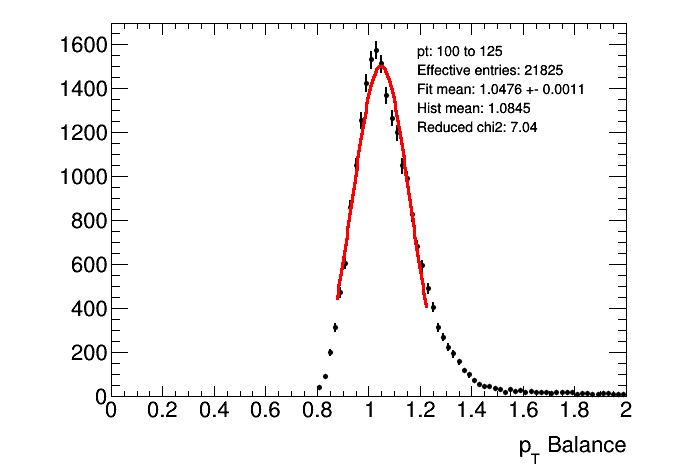
\includegraphics[width=0.31\textwidth]{plots/insitu/fits_data_zee_nominal/Zeejet_Nominal_Bin0.png}
    %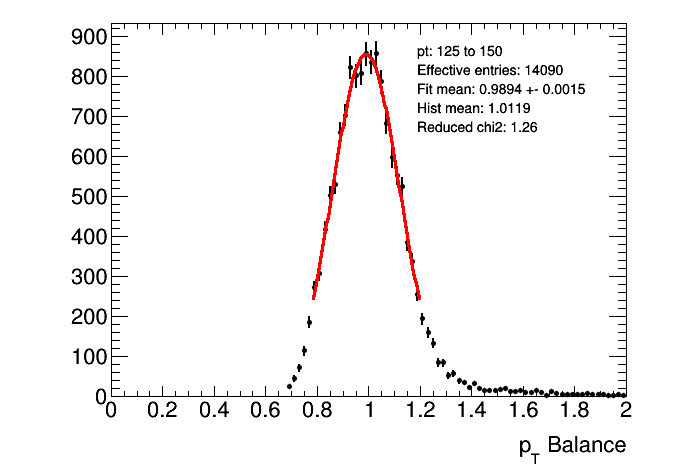
\includegraphics[width=0.31\textwidth]{plots/insitu/fits_data_zee_nominal/Zeejet_Nominal_Bin1.png}
    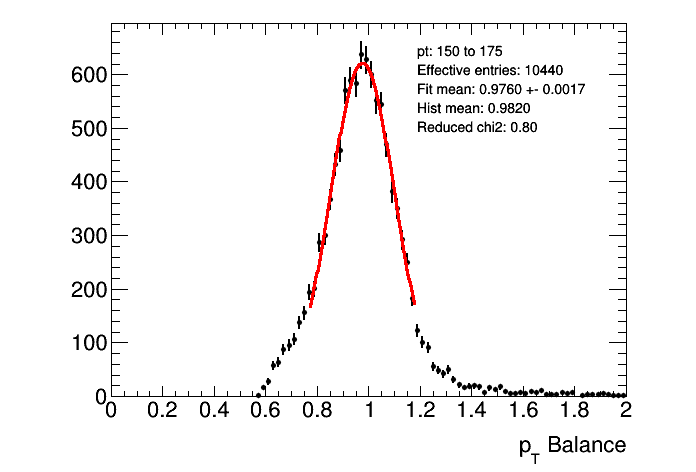
\includegraphics[width=0.31\textwidth]{plots/insitu/fits_data_zee_nominal/Zeejet_Nominal_Bin2.png}
    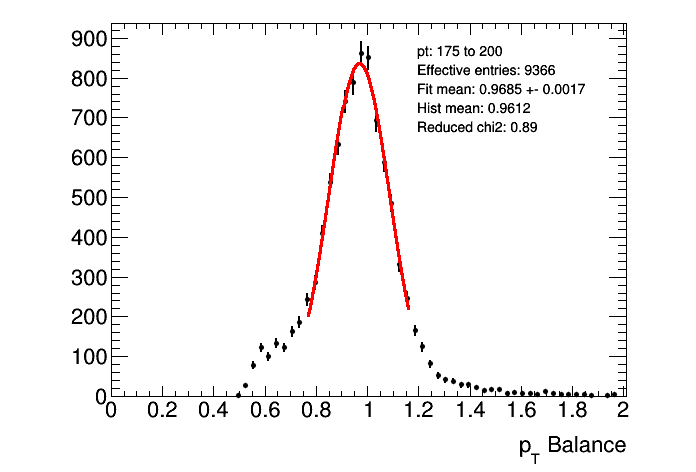
\includegraphics[width=0.31\textwidth]{plots/insitu/fits_data_zee_nominal/Zeejet_Nominal_Bin3.png}
    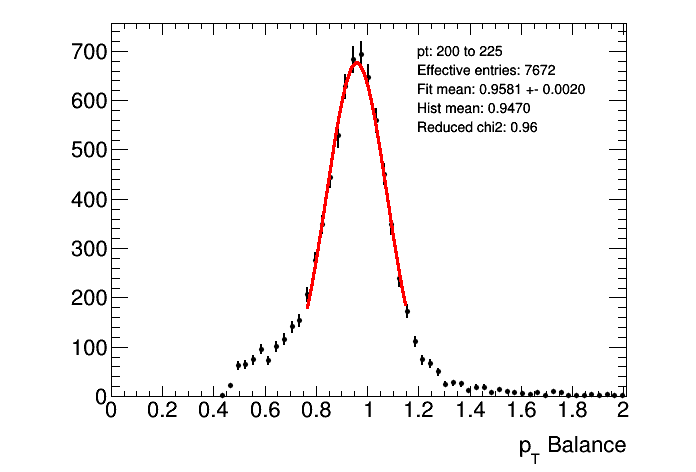
\includegraphics[width=0.31\textwidth]{plots/insitu/fits_data_zee_nominal/Zeejet_Nominal_Bin4.png}
    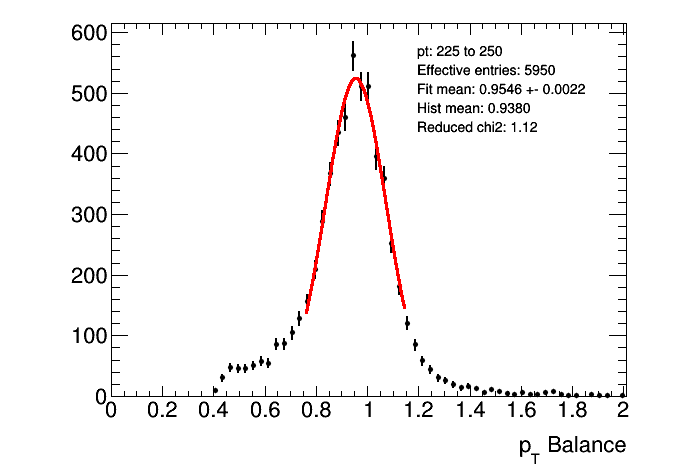
\includegraphics[width=0.31\textwidth]{plots/insitu/fits_data_zee_nominal/Zeejet_Nominal_Bin5.png}
    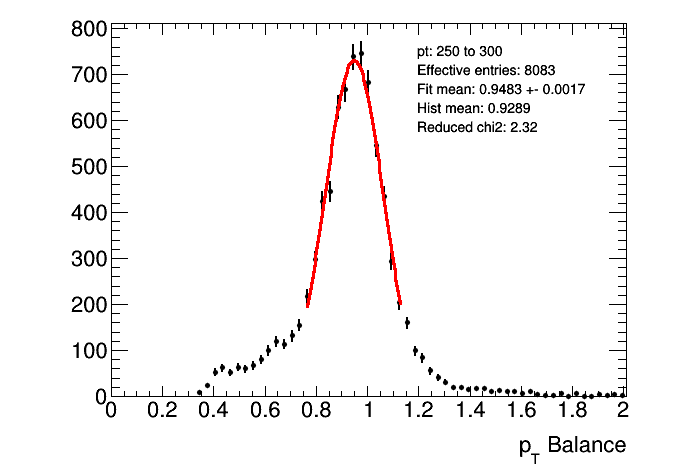
\includegraphics[width=0.31\textwidth]{plots/insitu/fits_data_zee_nominal/Zeejet_Nominal_Bin6.png}
    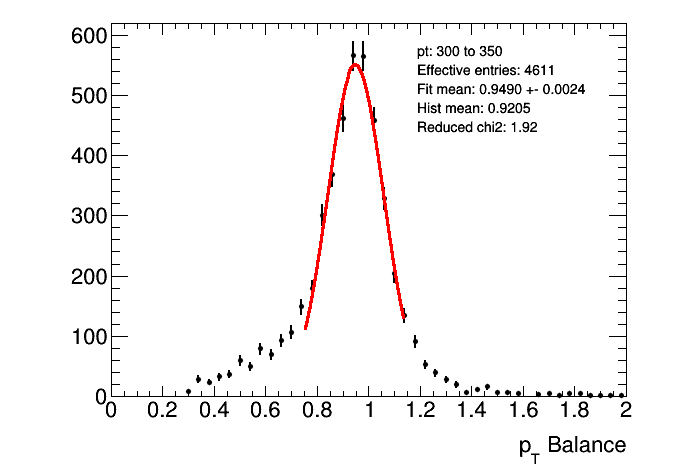
\includegraphics[width=0.31\textwidth]{plots/insitu/fits_data_zee_nominal/Zeejet_Nominal_Bin7.png}
    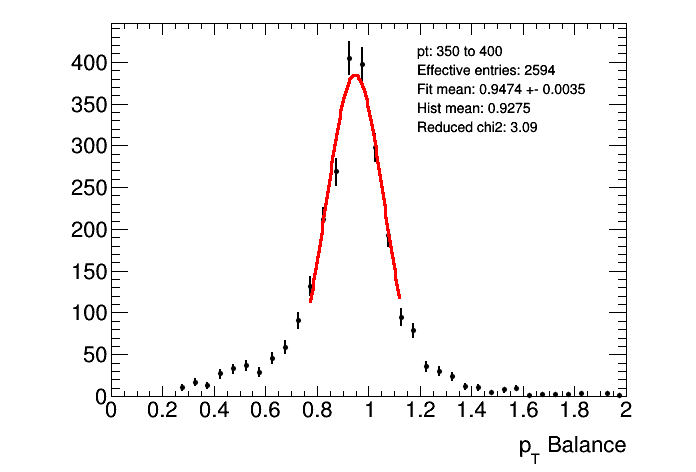
\includegraphics[width=0.31\textwidth]{plots/insitu/fits_data_zee_nominal/Zeejet_Nominal_Bin8.png}
    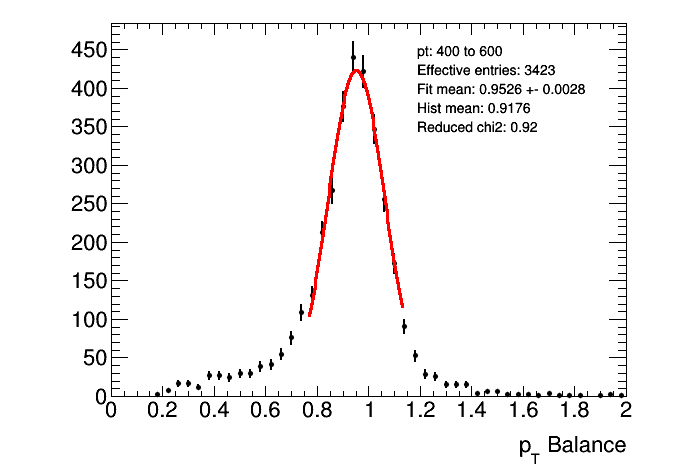
\includegraphics[width=0.31\textwidth]{plots/insitu/fits_data_zee_nominal/Zeejet_Nominal_Bin9.png}
    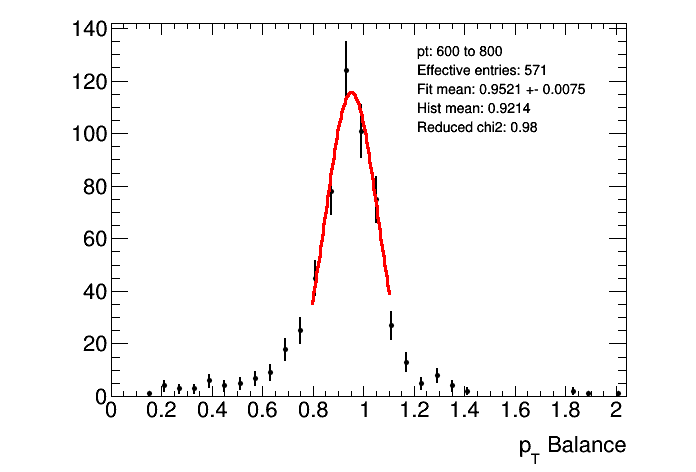
\includegraphics[width=0.31\textwidth]{plots/insitu/fits_data_zee_nominal/Zeejet_Nominal_Bin10.png}
    \caption{Gaussian fits to \ptbal in slices of \ptref in the electron channel. The $y$-axis shows the number of events per bin.\label{fig:insitu:zeedatafits}}
\end{figure}

\begin{figure}[t]
    \centering
    %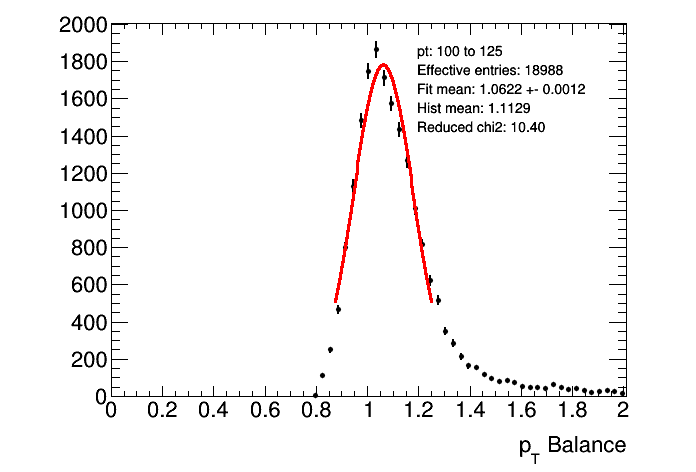
\includegraphics[width=0.31\textwidth]{plots/insitu/fits_data_zmm_nominal/Zmmjet_Nominal_Bin0.png}
    %\includegraphics[width=0.31\textwidth]{plots/insitu/fits_data_zmm_nominal/Zmmjet_Nominal_bin1.png}
    \includegraphics[width=0.31\textwidth]{plots/insitu/fits_data_zmm_nominal/Zmmjet_Nominal_bin2.png}
    \includegraphics[width=0.31\textwidth]{plots/insitu/fits_data_zmm_nominal/Zmmjet_Nominal_bin3.png}
    \includegraphics[width=0.31\textwidth]{plots/insitu/fits_data_zmm_nominal/Zmmjet_Nominal_bin4.png}
    \includegraphics[width=0.31\textwidth]{plots/insitu/fits_data_zmm_nominal/Zmmjet_Nominal_bin5.png}
    \includegraphics[width=0.31\textwidth]{plots/insitu/fits_data_zmm_nominal/Zmmjet_Nominal_bin6.png}
    \includegraphics[width=0.31\textwidth]{plots/insitu/fits_data_zmm_nominal/Zmmjet_Nominal_bin7.png}
    \includegraphics[width=0.31\textwidth]{plots/insitu/fits_data_zmm_nominal/Zmmjet_Nominal_bin8.png}
    \includegraphics[width=0.31\textwidth]{plots/insitu/fits_data_zmm_nominal/Zmmjet_Nominal_bin9.png}
    \includegraphics[width=0.31\textwidth]{plots/insitu/fits_data_zmm_nominal/Zmmjet_Nominal_bin10.png}
    \caption{Gaussian fits to \ptbal in slices of \ptref in the muon channel. The $y$-axis shows the number of events per bin.\label{fig:insitu:zmmdatafits}}
\end{figure} %%%HERE%%%

The 18 Gaussian fits in Figures \ref{fig:insitu:zeedatafits} and \ref{fig:insitu:zmmdatafits} qualify the average jet response, \rdb, as a function of \ptref. However, since the final insitu calibration is applied to large-R jets, the \ptref values need to be mapped to \ptJ. To derive the mapping, a 2D histogram of \ptref vs \ptJ is produced. For a given \ptref slice, the \ptJ bin center is given by the histogram mean over the range $[0.4p_{\text{T,ref},i}^{\text{low}},1.6p_{\text{T,ref},i}^{\text{high}}]$, where $p_{\text{T,ref},i}^{\text{low}}$ and $p_{\text{T,ref},i}^{\text{high}}$, are the lower and upper bin edges for bin $i$ of \ptref, respectively. The $\ptJ$ midpoint values for each \ptref bin are shown in Figure \ref{fig:insitu:mapping}.
\begin{figure}[t]
\centering
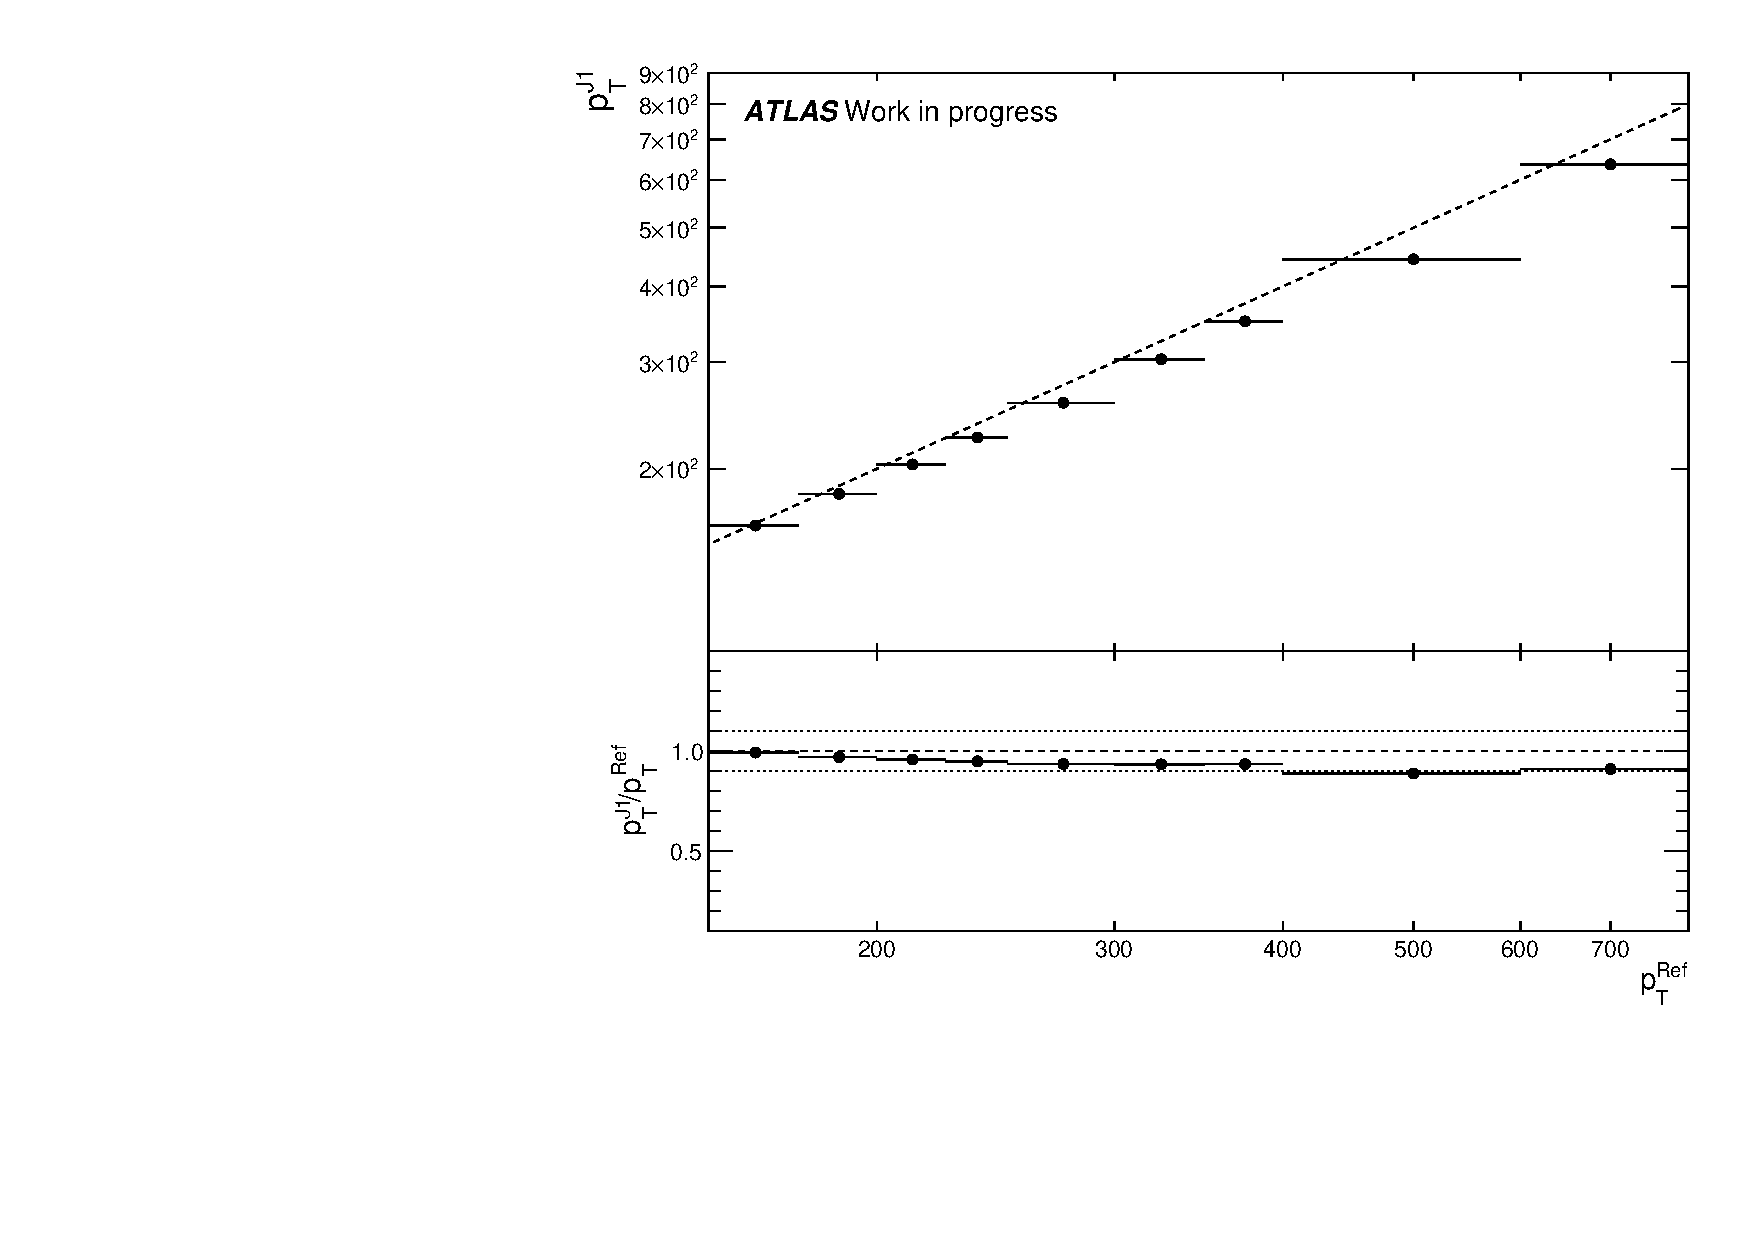
\includegraphics[width=\textwidth]{plots/insitu/Sherpa.all_MappingVsPt_WIP.pdf}    
\caption{\ptref with midpoint \ptJ values on a log scale. The horizontal bars represent the bin edges of the original \ptref binning. The black dots in the top canvas shows the $\ptJ$ midpoints for a given \ptref slice. The diagonal line is $\ptJ = \ptref$. The ratio plot shows the ratio of the midpoints of the \ptJ bins with the midpoints of the \ptref bins. It is evident from this plot that the bins at higher \ptref have a larger correction than the bins at lower \ptref.\label{fig:insitu:mapping}}
\end{figure}

%\clearpage
\section{Systematic Uncertainties}

Systematic uncertainties in the insitu correction arise from the reconstruction and calibration of the leptons, the choice of event generator used to calculate the double ratio $c$, the JVT working point, and the variations in the event selection criteria (given in Table \ref{tab:evsel_insitu}). JES and JER systematic uncertainties on the small-R jet used in the radiation veto, and lepton reconstruction, ID, isolation and trigger efficiency scale factors, are not considered. These uncertainties were found to be negligible in previous large-R jet calibration efforts at ATLAS \cite{Atlas:largercali}. The statistical uncertainties from the number events in data, and the number of simulated events are included in the final uncertainty. 

There are 64 independent sources of uncertainty which contribute to the electron energy scale variations. These include uncertainties in the material upstream of the calorimeter, cell readout non-linearity, transitions between higher and lower gains in the EM calorimeter, presampler calibration, intercalibration of first and second accordion layers, \zee energy scale calibration, pileup modelling, and lateral shower shape development \cite{Atlas:egamcal_fullrun2}. 

The sources of uncertainty contributing to the electron energy resolution are: shower and sampling variations in the calorimeter, fluctuations in the energy loss upstream of the calorimeter, electronics and pileup noise, and residual non-uniformities affecting the measurement of the energy in the data \cite{Atlas:egamcal_run2}. For the muon \pt scale and resolution uncertainties, the sources include: the $J/\psi\rightarrow\mu^+\mu^-$ and \zmm fits, reweighting simulated $Z$ samples to improve agreement with data, decay and final state radiation modelling, $J/\psi/Z$ \pt template range, $J/\psi/Z$ mass binning, $J/\psi/Z$ mass window, $J/\psi$ alternate background parametrisation function, the closure test, and statistical uncertainty \cite{Insitu:muoncal}.

%
%\begin{itemize}
%    \item Uncertainties in the material upstream of the calorimeter,
%    \item Cell readout non-linearity,
%    \item Transitions between higher and lower gains in the EM calorimeter,
%    \item Presampler calibration,
%    \item Intercalibration of first and second accordion layers,
%    \item \zee energy scale calibration uncertainties,
%    \item Pileup modelling,
%    \item Lateral shower shape development.
%\end{itemize}
%The contributions to the electron energy resolution are \cite{Atlas:egamcal_run2}:
%\begin{itemize}
%    \item Shower and sampling variations in the calorimeter,
%    \item Fluctuations in the energy loss upstream of the calorimeter,
%    \item Uncertainties from the electronics and pileup noise,
%    \item Residual non-uniformities affecting the measurement of the energy in the data.
%\end{itemize}
%The sources of uncertainty contributing to the muon \pt scale and resolution are \cite{Insitu:muoncal}:
%\begin{itemize}
%    \item Uncertainties from the $J/\psi\rightarrow\mu\mu$ and $Z\rightarrow\mu\mu$ fits,
%    \item Uncertainties from reweighting simulated $Z$ samples to improve agreement with data,
%    \item Decay and final state radiation modelling,
%    \item $J/\psi/Z$ \pt template range,
%    \item $J/\psi/Z$ mass binning,
%    \item $J/\psi/Z$ mass window,
%    \item $J/\psi$ alternate background parametrisation function,
%    \item Closure test and statistical uncertainty.
%\end{itemize} 
 Up and down variations in the each of the scale and resolution systematic uncertainties are propagated independently through the analysis chain and are later symmetrised (with the exception of MC modelling and JVT). Systematic variations in the electron and muon calibration are applied only to simulation when calculating the systematic uncertainty on the double ratio $c$. Each source of uncertainty for the $e/\mu$ scale and resolution is considered as fully correlated across $\eta$ and $\pt$, and are all added in quadrature (independently for electrons, and MS and ID components for muons)

The MC modelling uncertainty is evaluated by performing the response measurements separately for the \SHERPA and \POWPY samples. The double ratio is calculated for both response measurements, and the difference between the nominal values defines the uncertainty. Sherpa is chosen as the nominal MC generator because a significantly larger degree of mismodelling is seen in the Powheg-Pythia samples as a function of jet \pt as shown in Figure \ref{fig:insitu:mismodelling}.
\begin{figure}[t]
\centering
\begin{subfigure}[b]{0.48\textwidth}
    \centering
    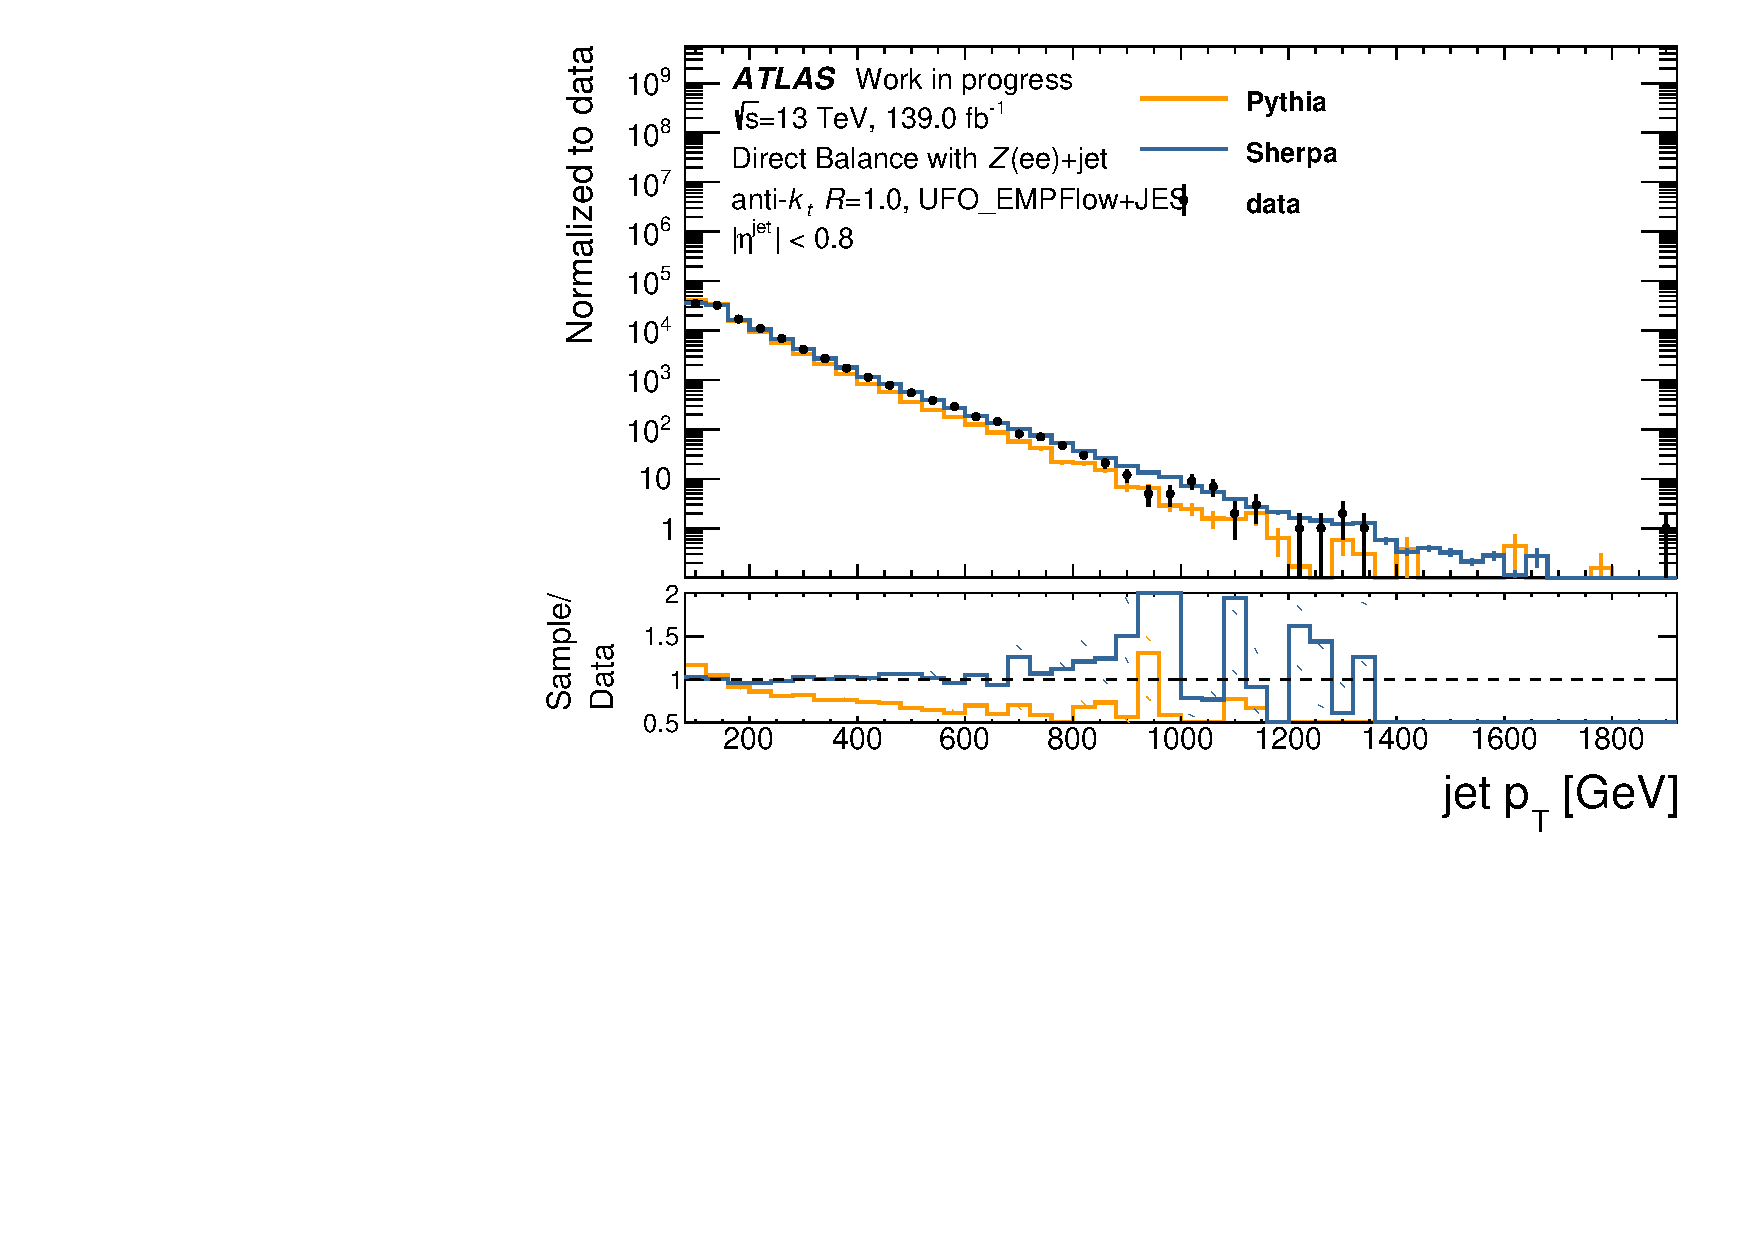
\includegraphics[width=\textwidth]{plots/insitu/Zeejet_Nominal_jetPt_jet0_logY.pdf}
    \caption{}
    \label{fig:insitupt:a}
\end{subfigure}
\hfill
\begin{subfigure}[b]{0.48\textwidth}
    \centering
    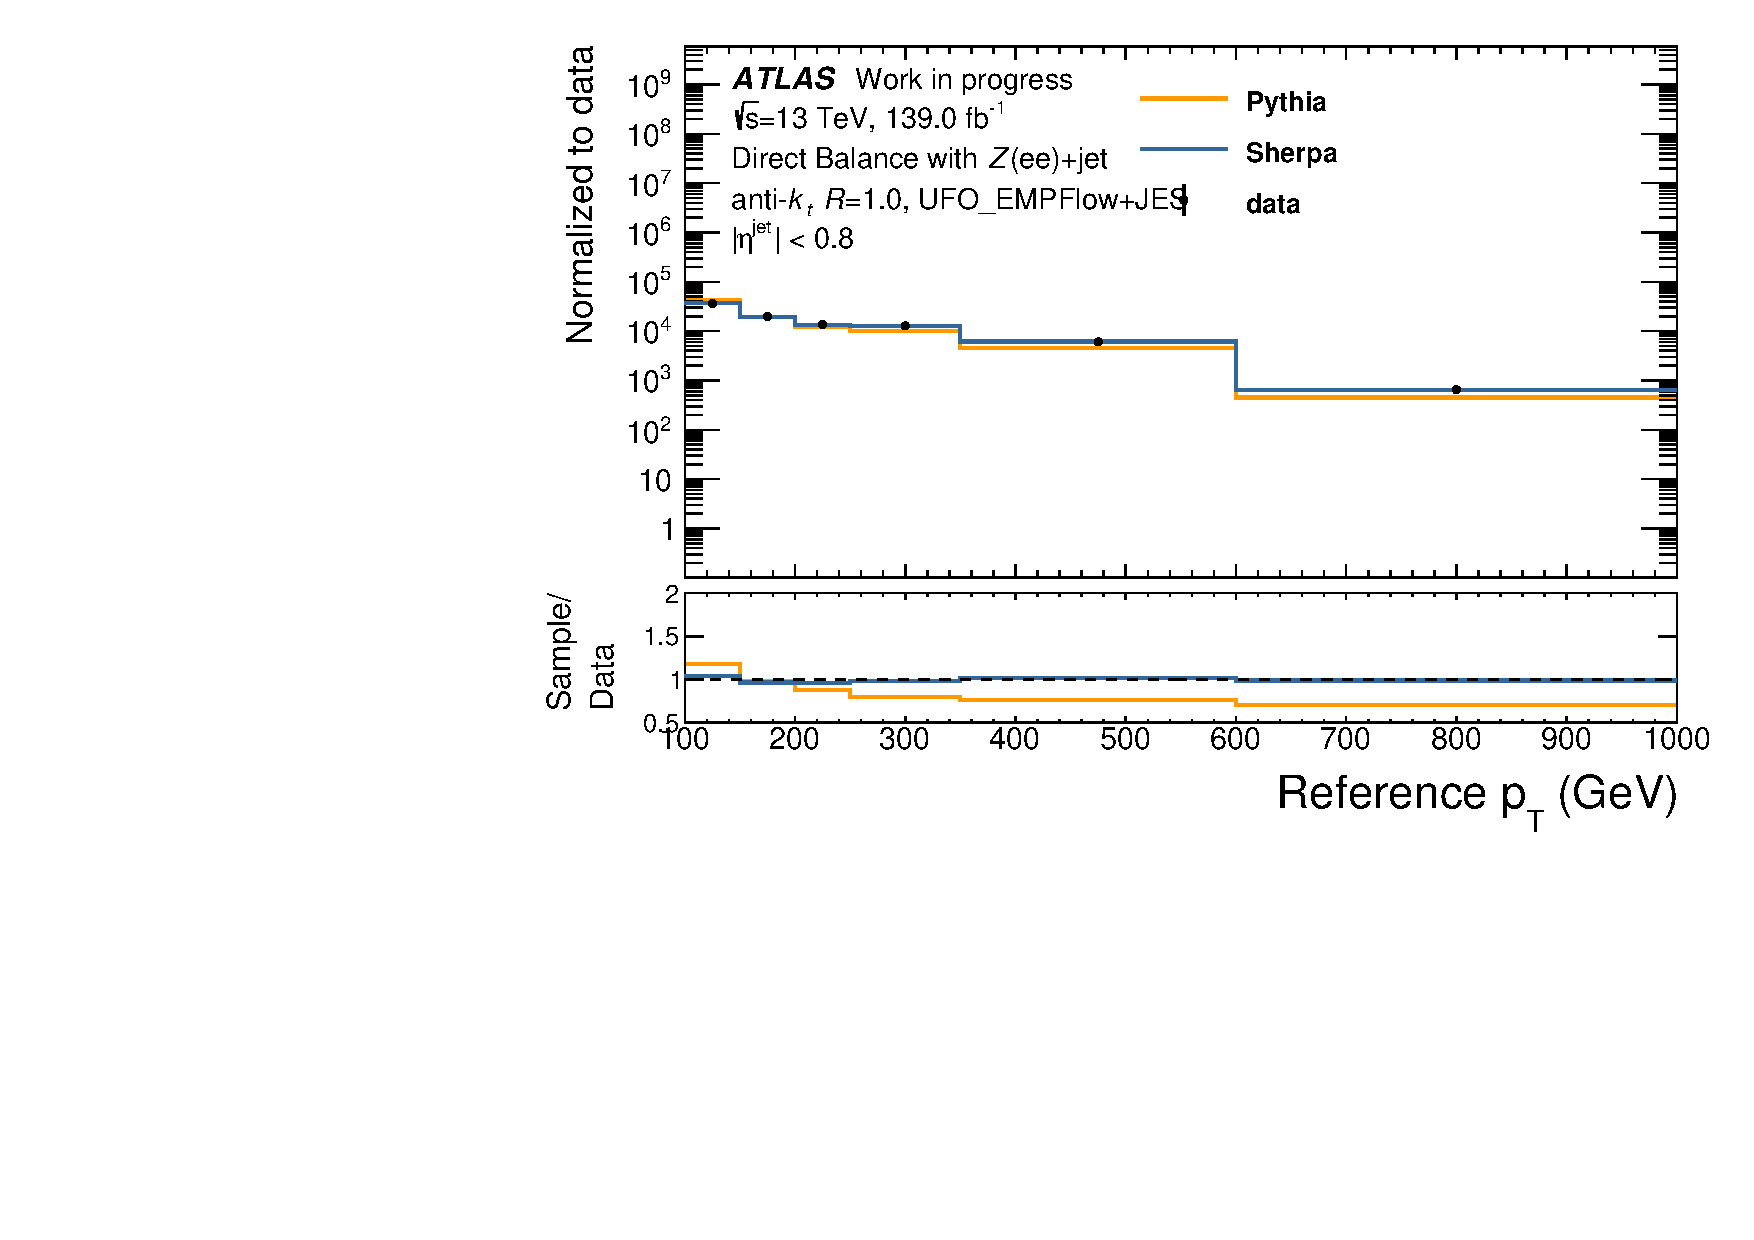
\includegraphics[width=\textwidth]{plots/insitu/Zeejet_Nominal_refPt_logY.pdf}
    \caption{}
    \label{fig:insitupt:b}
\end{subfigure}
\caption{Data to MC distributions for the \ptJ (a) and \ptref (b). The MC distributions are normalised to the data distribution. It is clear that there is a large degree of mismodelling in the \POWPY MC sample which cannot be explained by the lack of an insitu calibration, as this is of the order of a few \%. For this reason the \POWPY sample is only used to quantify a systematic modelling uncertainty of $c$, and is not used in the calculation of the nominal value.\label{fig:insitu:mismodelling}}%From MJB documentation: NLO Powheg+Pythia 8 was known to have an issue matching jets with the parton shower, leading to poor modeling of all jet pT, as well as the recoil system pT, as seen in Figure 2 a, c, d.
\end{figure}

For uncertainties associate with JVT, the \textit{Medium} working point is used. The default \textit{Tight} working point is defined by the threshold $JVT > 0.5$, and the \textit{Medium} working point is $JVT > 0.2$. The cut values refer to the output values of the JVT likelihood-based discriminant derived from simulated dijet events \cite{Insitu:JVT}.

Systematic variations in the event selection criteria are carried out to test the assumption of a $2\rightarrow2$ topology. The $\Delta\phi(J,Z)$ variations are defined by varying the default selection by $\pm0.1$ radians. Table \ref{tab:evsel_insitu} gives the variations in the radiation veto. Event selection and JVT systematic variations are performed simultaneously in data and MC. 

Each source of uncertainty is considered as fully correlated across $\eta$ and \pt. Each uncertainty is evaluated by propagating each source through the analysis chain and calculating its effect on the double ratio, $c$. The final uncertainty is taken to be the quadrature sum of the individual uncertainties.

%The statistical uncertainties on in data and MC responses are given by the standard error on the mean of the Gaussian fits, i.e. $\sigma/\sqrt{N}$, where $\sigma$ is the fitted standard deviation, and $N$ is the number of data or MC events. The data and MC statistical uncertainties are propagated to the \rdb using error propagation for uncorrelated uncertainties.
% 1. Discuss how the e/mu/jvt uncertainties are defined and talk about up and down variations and symmetrising
% 2. Include a cutflow, NAH
% 3. Discuss the bootstrapping, show an example of the bootstrapping, maybe generator choice.

%The \textit{bootstrapping} procedure is used to evaluate the statistical significance of the systematic uncertainties.    This is done such that one can separate contributions from statistics and systematics in the following way. Consider one set MC events where, for example the Jet Energy Scale (JES), is at its nominal value and another set of events where the JES is at a slightly different value, the events remain entirely correlated, one just has a slightly different scaling for the jet energies and \pt. One of the implications of this is that if one wants to determine the statistical uncertainty \textbf{on a} systematic uncertainty (derived by subtracting the extracted yields from using nominal and varied templates), that the standard error propagation formalism cannot be used (this assumes uncorrelated uncertainties). One way to approach this problem is through the \textit{bootstrapping} procedure, where $N_{\text{bootstraps}}$ pseudo-experiments are constructed for the nominal case and for each systematic variation. These bootstraps are created by multiplying each MC event weight by a random number sampled from a unit (discrete) Poisson distribution. The bootstraps are created in such a way as to preserve the correlations between nominal bootstrap numbered $x$, and systematic bootstrap corresponding to the same number, $x$. If these correlations we not preserved, the difference between the nominal and systematic bootstraps would not just correspond to the difference due to the systematic variation, but also due to the statistical variations between each bootstrap, hence the resulting statistical uncertainty would be drastically overestimated. The correlations are preserved by choosing the same random number seed when sampling the unit Poisson for each nominal and systematic MC event corresponding to the same event number. $N_{\text{bootstraps}}=10000$ is determined to be sufficient for this analysis.%Since the MC and data stat uncertainties are the largest uncertainties on the measurement, it is impotartant that a sufficient number of bootstraps is used to determine these precisely. 
%
%The systematic uncertainties provide information about real changes in the response due to changes in the MC event generator, physics objects, and event selection definitions. However, the response can also change solely because a different statistically random set of events was selected. It is therefore a requirement that the systematic uncertainties should be statistically significant, i.e. there is a small probably -- less than $4.55\%$ in our case -- that the changes in the response come about solely due to random statistical fluctuations.

To prevent large statistical fluctuations in the systematic uncertainties, a \textit{bootstrapping} procedure is used to determine a statistically significant re-binning for every source of uncertainty. In this procedure, 100 bootstrap replicas are created, where each replica has a copy of the nominal 2D distribution (Figure \ref{fig:insitu:2dhistzeedata}) and each systematically varied 2D distribution. For each event in the dataset, 100 event weights are chosen by sampling a Poisson distribution with mean of one. These represent a modified set of event weights, one for each bootstrap replica. Each replica histogram is then filled with its corresponding set of event weights. The sampling of the Poisson distribution depends on a random number uniquely determined from the run and event number. In this way, nominal events, and events corresponding to systematic variations remain correlated for every replica. The nominal \rdb response values for one of the \ptref bins in data for 100 replicas is shown in Figure \ref{fig:insitu:replicas}.

%In this procedure, a pseudodataset called a ``replica'' is also filled with each event weight multiplied by an integer factor sampled from a unit Poisson distribution. 100 such replicas are filled, and the collection of replicas defines a ``bootstrap'' object. A bootstrap object is created for the nominal dataset and for each systematic variation. For each event replica, the sampling of the Poisson distribution depends on a random number uniquely determined from the run and event number. In this way, nominal events, and events corresponding to systematic variations remain correlated for every replica in the bootstrap. The bootstrapping is used to derive a statistically significant re-binning for the systematic uncertainties, it does not have a large effect on the values themselves. The distribution of fitted \rdb response values for one of the \ptref bins in data for \zee events is shown in Figure \ref{fig:insitu:replicas}.
\begin{figure}[t]
\centering
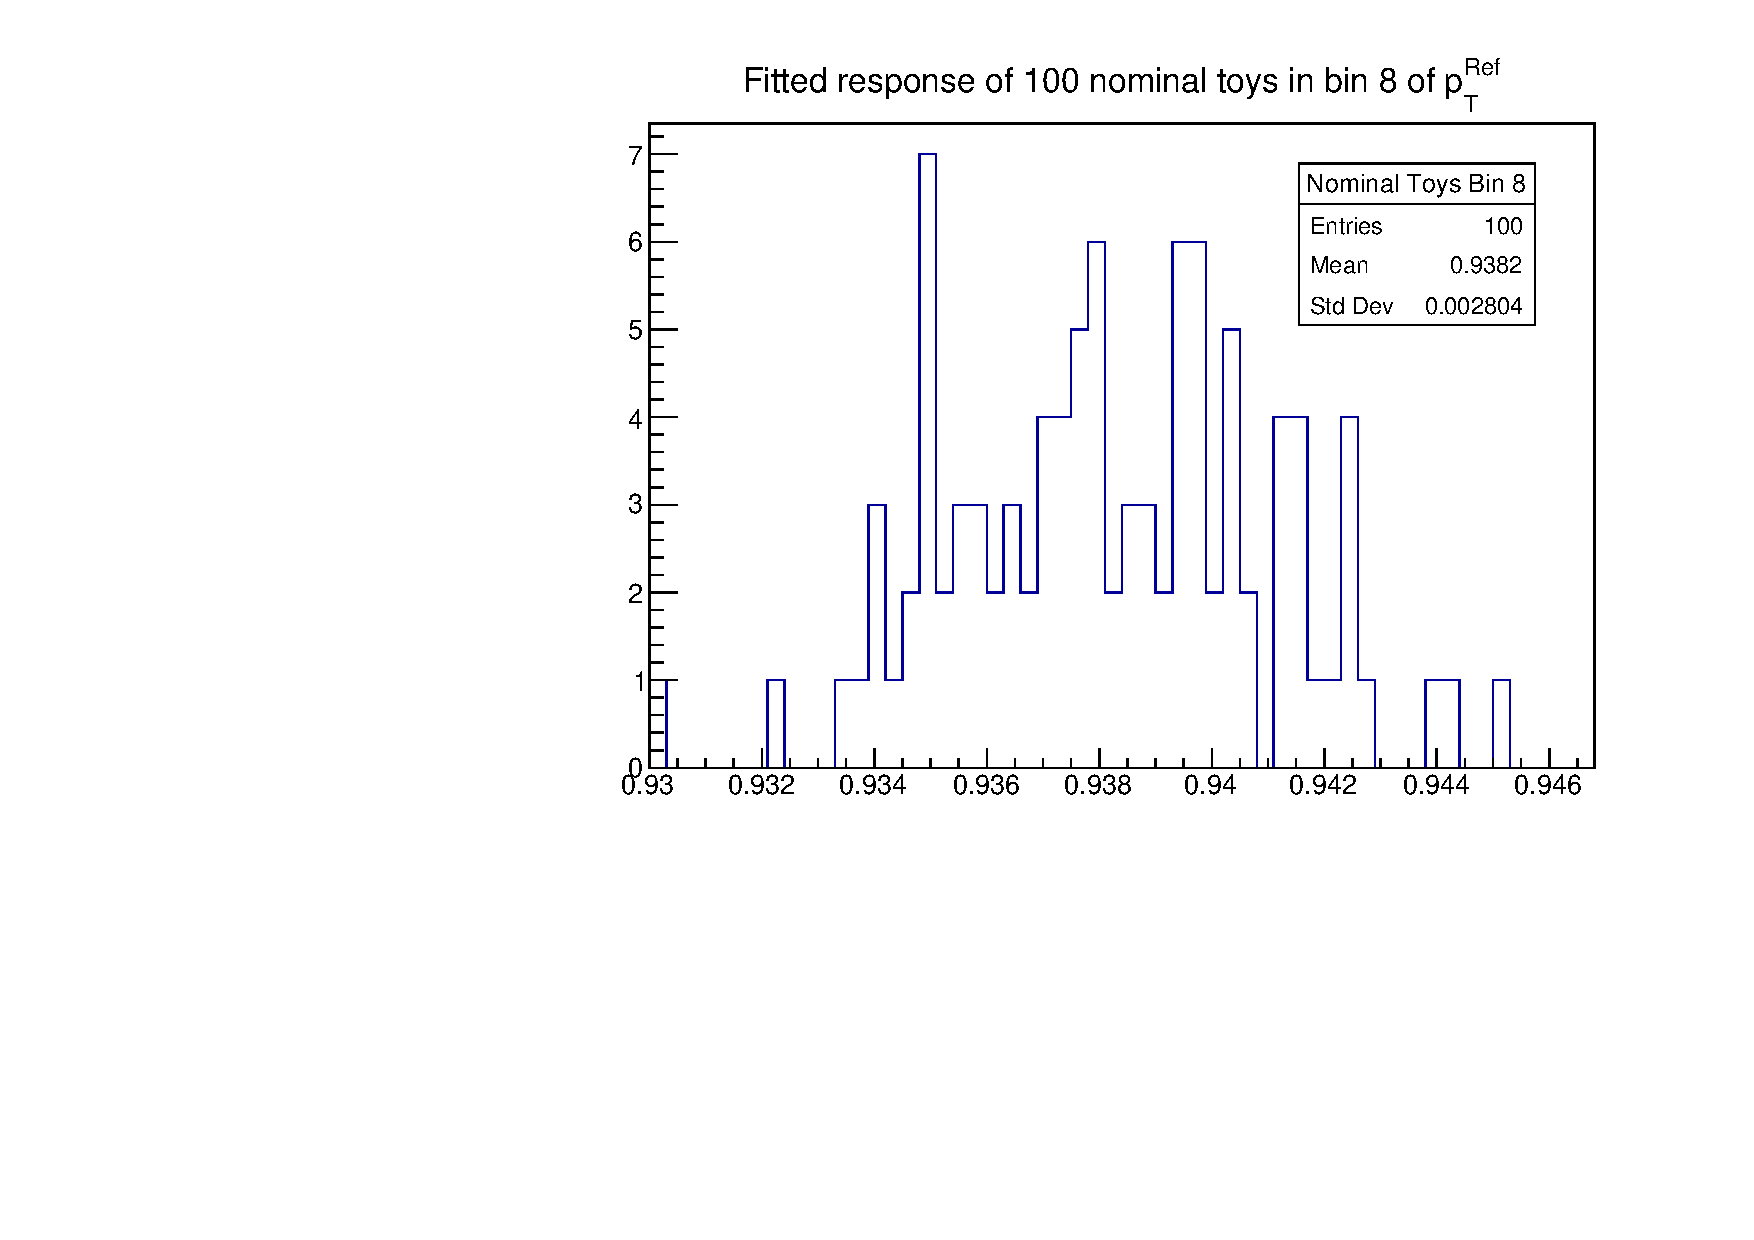
\includegraphics[width=0.8\textwidth]{plots/insitu/Nominal_response_toys_bin8.pdf}
\caption{The \rdb response derived from 100 nominal replica distributions in bin 8 of \ptref in the electron channel. Every entry in this histogram has a corresponding value for any given systematic uncertainty. By calculating the spread in the differences between these correlated values, the statistical significance of the systematic variation for a given bin can be ascertained. The $x$-axis shows \ptref and the $y$-axis shows the number of replica instances per bin.\label{fig:insitu:replicas}}
\end{figure}

The re-binning procedure works by iterating over each \ptref bin, and determining the double ratio $c$ for each replica of the systematic variation ($c_{i}^{\text{sys}}$), and for each nominal replica ($c_{i}^{\text{nom}}$). The value of the systematic uncertainty for a given replica, $i$, is then given by: 
\begin{equation}
\delta_{\text{sys},i}=\frac{c_{i}^{\text{sys}}-c_{i}^{\text{nom}}}{c_{i}^{\text{nom}}}.
\end{equation}
The statistical significance of the systematic variation is given by the ratio of the systematic uncertainty calculated from the un-fluctuated dataset, $\delta_{\text{sys}}$, and the standard deviation of the replica systematic uncertainties. The systematic uncertainty is deemed to be statistically significant if this ratio is larger than 2. If this criteria is met, the bin is kept as it was. Otherwise, the \ptref bin is combined with the next bin, and the nominal and systematic responses are re-fit with the combined bins. If the significance threshold is still not reached, the next \ptref bin is added, and the responses are subsequently re-fit. To prevent over-binning, only a maximum of 5 bins are allowed to be combined. An example of a systematic uncertainty which is rebinned (MC modelling) and one which is not rebinned (electron energy scale) is shown in Figure \ref{fig:insitu:mctypescale}.

\begin{figure}[t]
\centering
\begin{subfigure}[b]{0.48\textwidth}
    \centering
    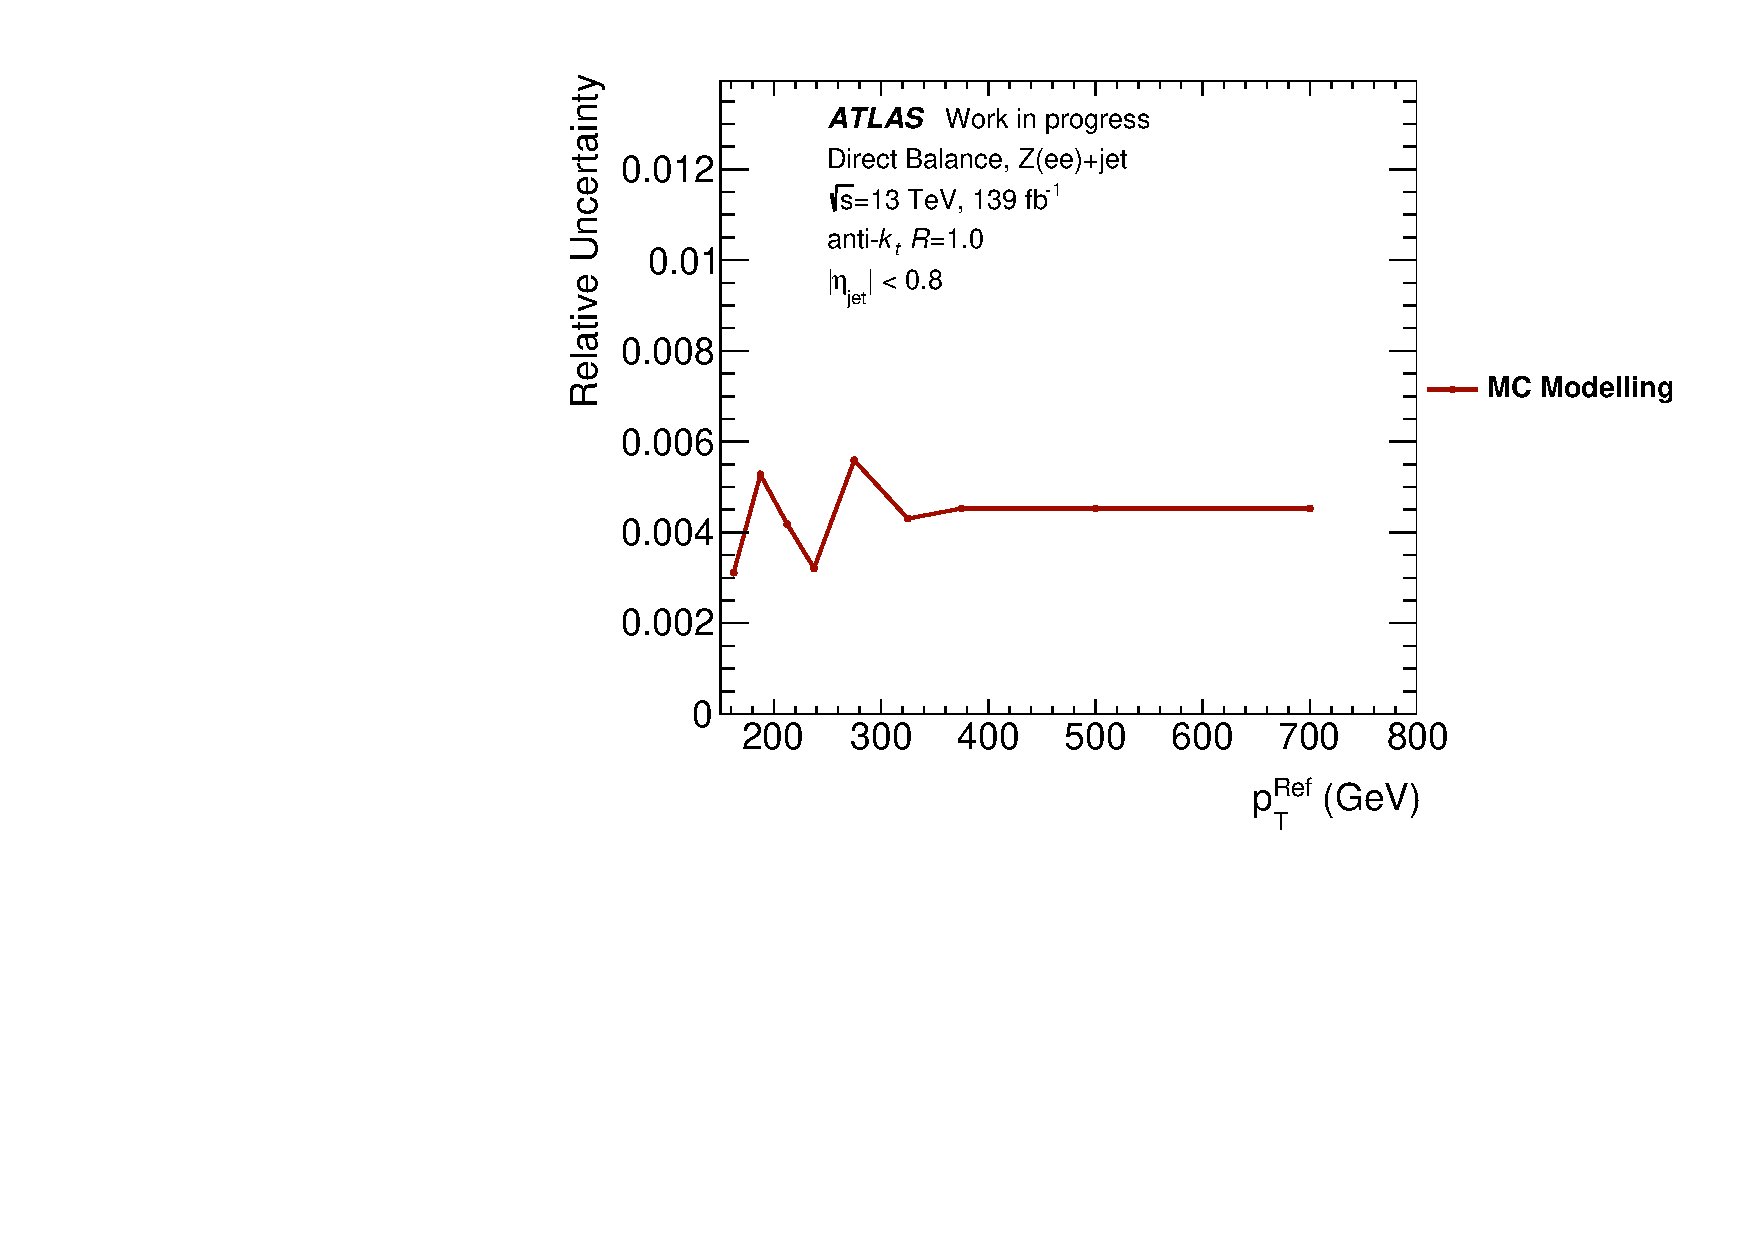
\includegraphics[width=\textwidth]{plots/insitu/mctype_WIP.pdf}
    \caption{}
    \label{fig:insitupt:a}
\label{fig:insitupt:a}
\end{subfigure}
\begin{subfigure}[b]{0.48\textwidth}
    \centering
    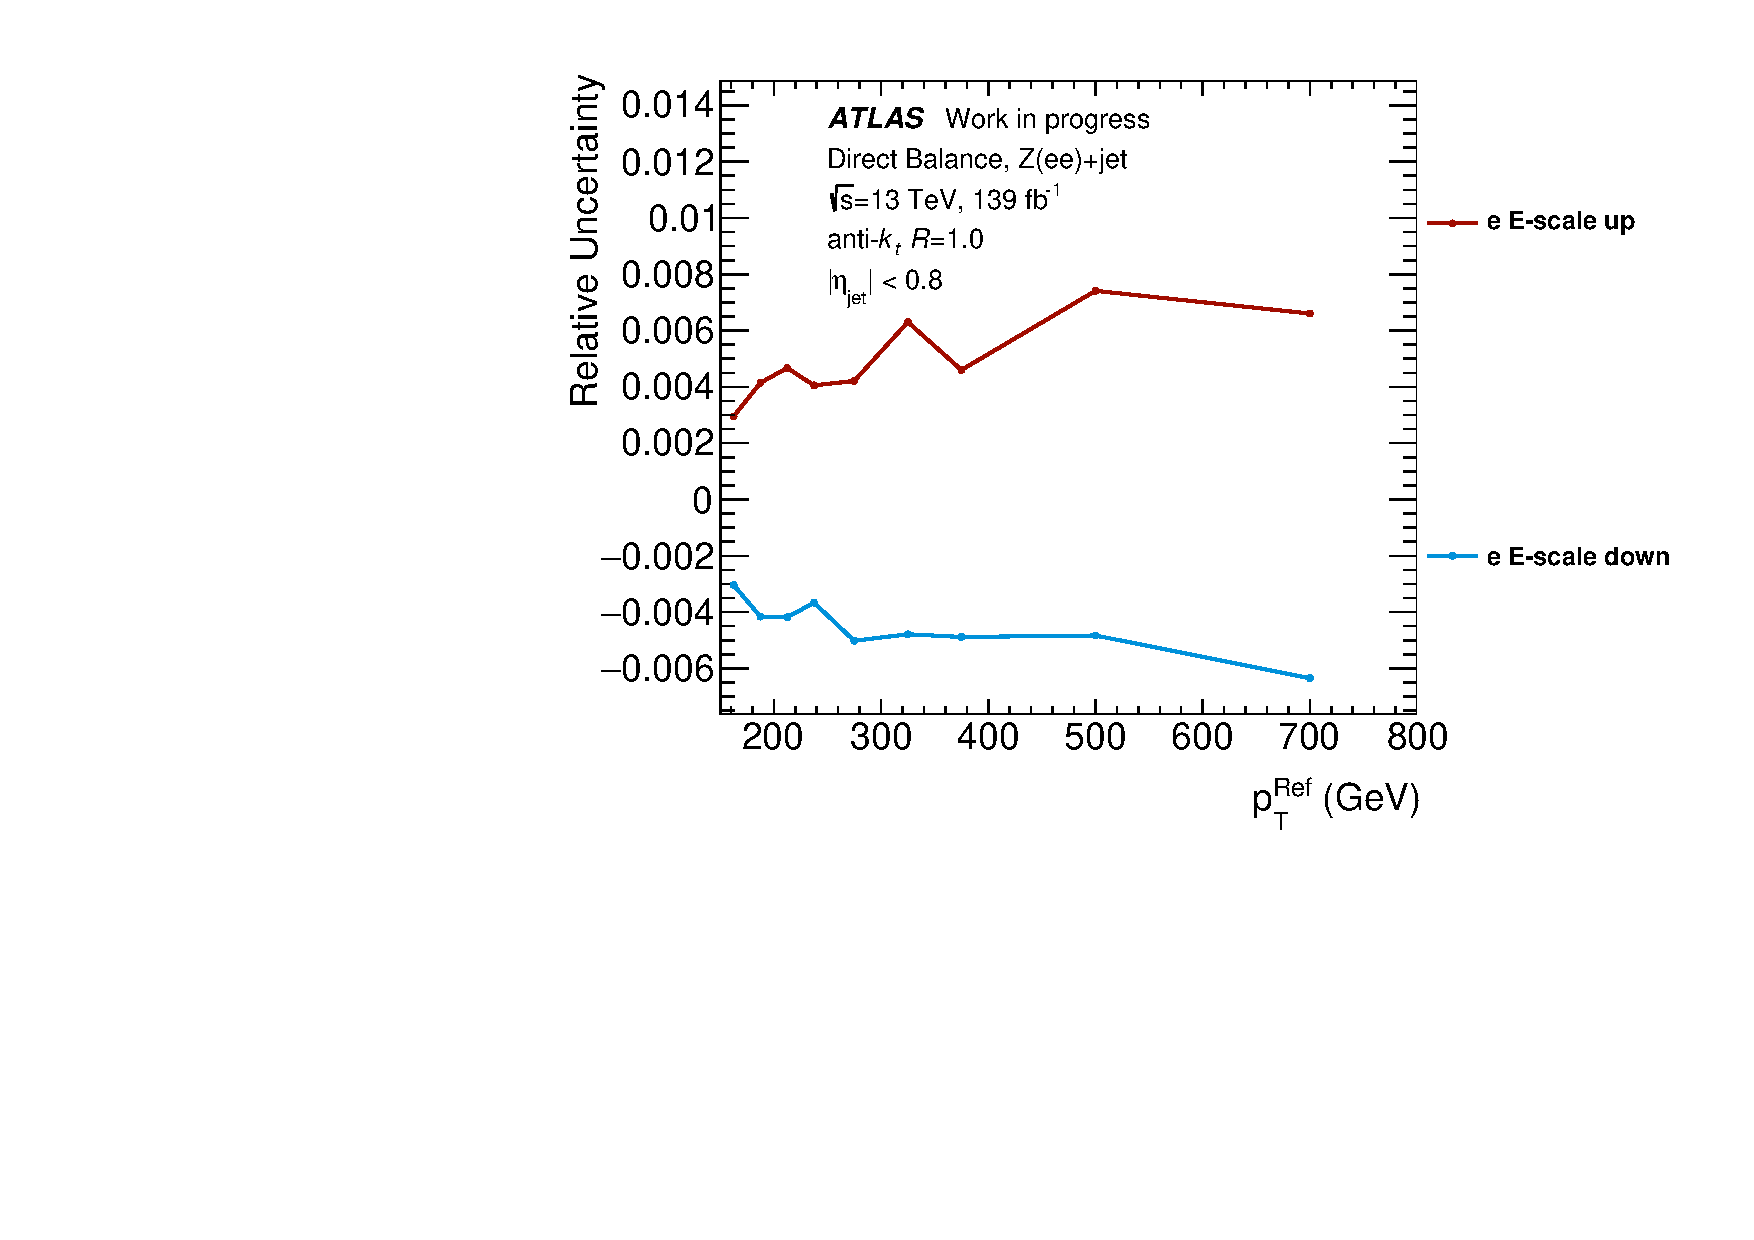
\includegraphics[width=\textwidth]{plots/insitu/egamma_scale_WIP.pdf}
    \caption{}
    \label{fig:insitupt:b}
\end{subfigure}
\hfill
\begin{subfigure}[b]{0.48\textwidth}
    \centering
    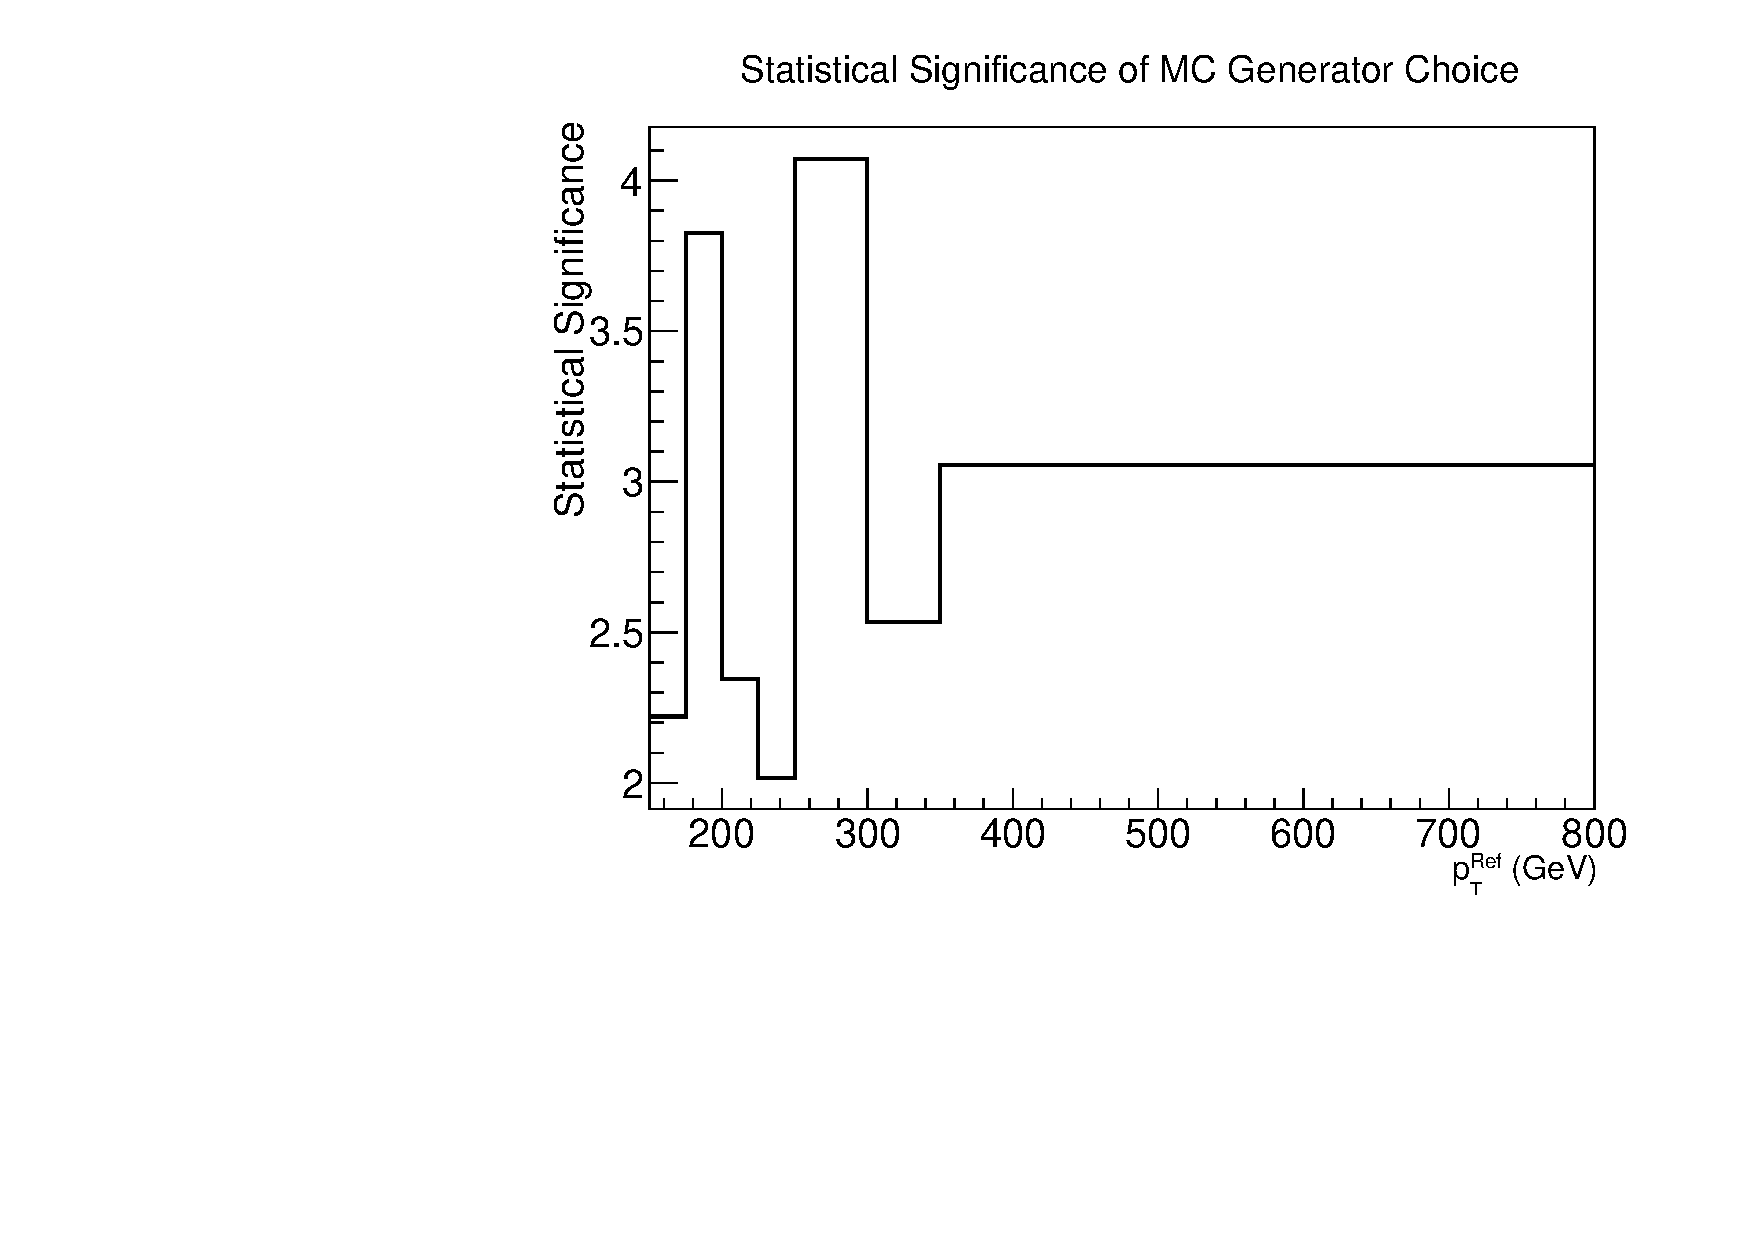
\includegraphics[width=\textwidth]{plots/insitu/mcchoice_sig.pdf}
    \caption{}
    \label{fig:insitupt:c}
\end{subfigure}
\begin{subfigure}[b]{0.48\textwidth}
    \centering
    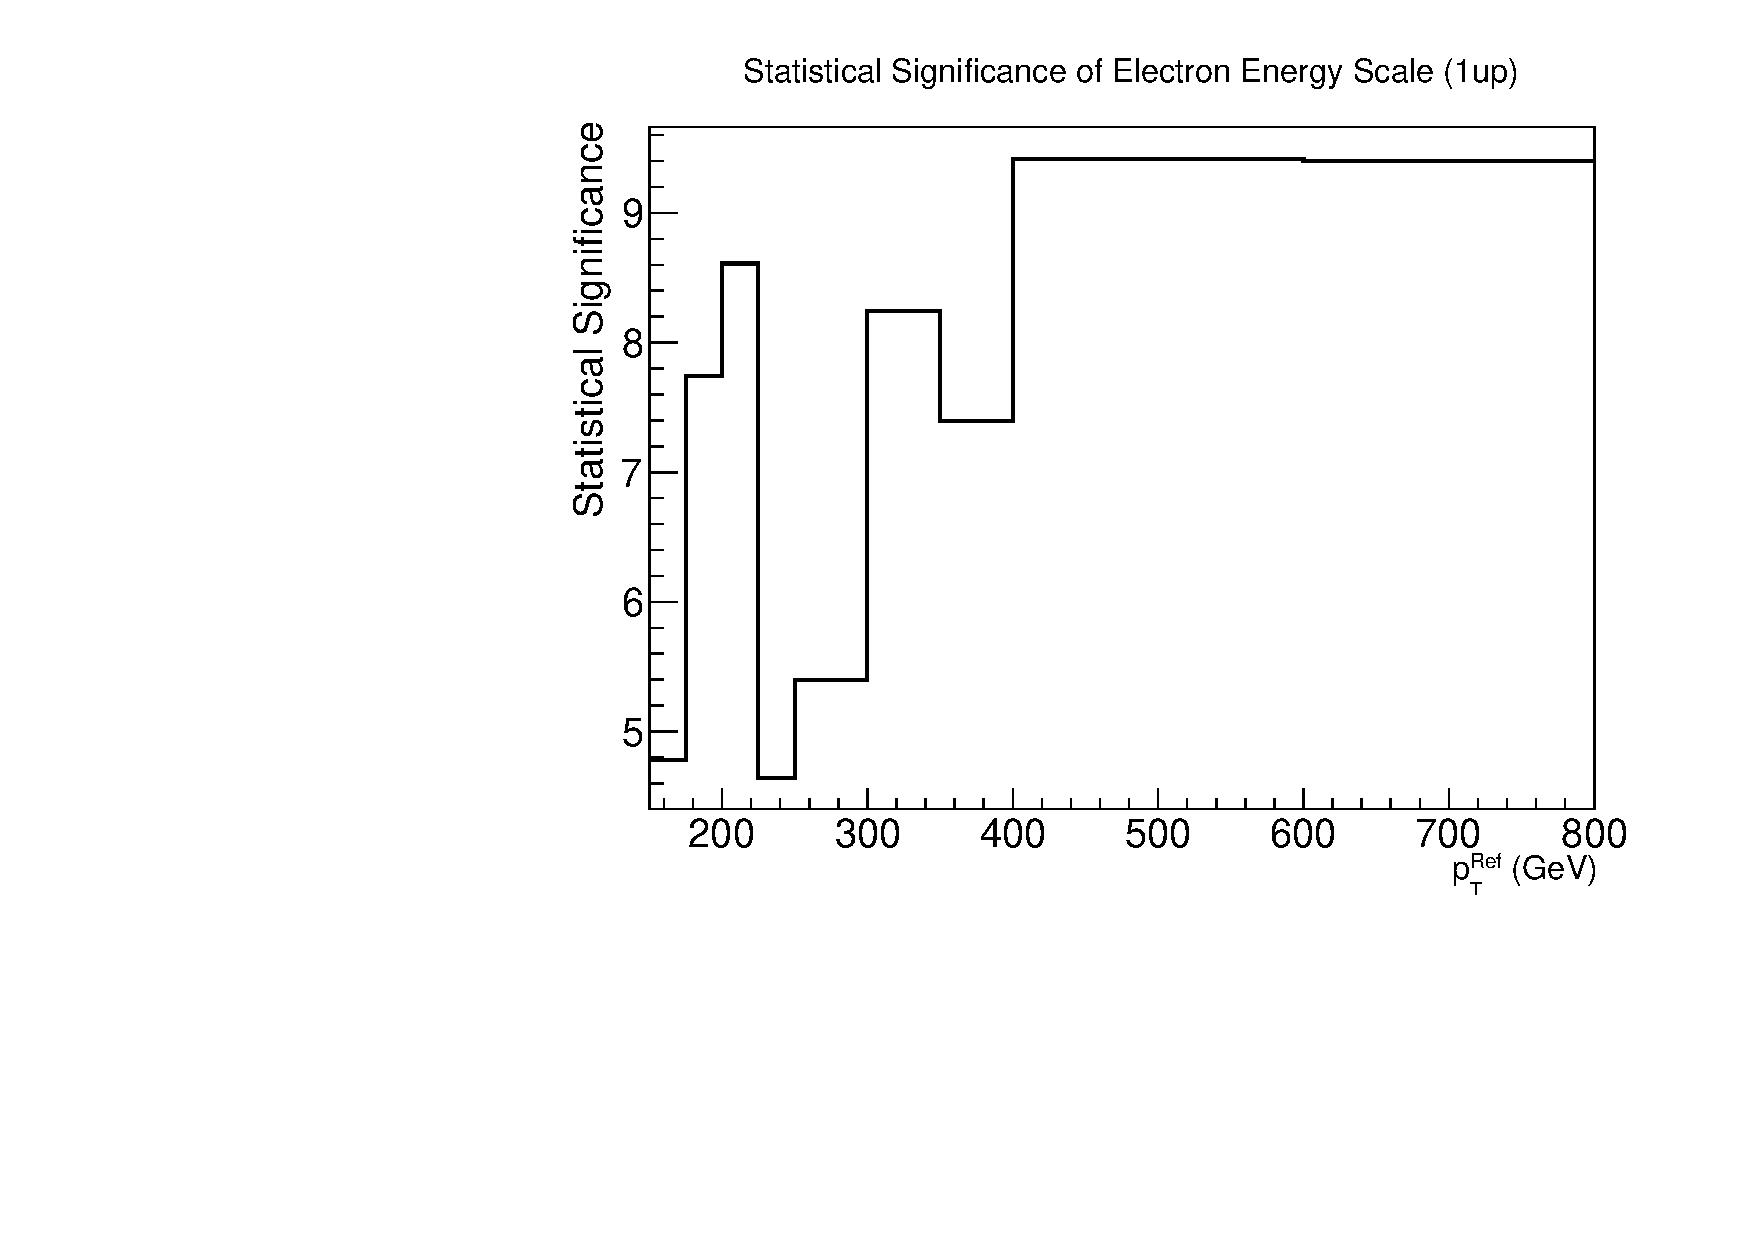
\includegraphics[width=\textwidth]{plots/insitu/eescale_sig.pdf}
    \caption{}
    \label{fig:insitupt:d}
\end{subfigure}
\caption{MC modelling uncertainty on \rdb prior to the mapping to \ptJ (a). Electron energy scale uncertainties on \rdb prior to mapping to \ptJ. Statistical significance of the MC modelling uncertainty is shown in (c), and the up variation of the electron energy scale in (d). In (a), the last two bins (bins 7 and 8) were not statistically significant, but were made statistically significant with the addition of bin 6. In (b), all uncombined bins are statistically significant, and no rebinning has taken place.\label{fig:insitu:mctypescale}}%From MJB documentation: NLO Powheg+Pythia 8 was known to have an issue matching jets with the parton shower, leading to poor modeling of all jet pT, as well as the recoil system pT, as seen in Figure 2 a, c, d.
\end{figure}

%(containing 100 replicas) of the 2D histogram response histograms (Figure \ref{fig:insitu:2dhistzeedata}) are created. To create the replicas, each event weight is multiplied by a random integer sampled from a unit Poisson distribution. The Poisson distribution is sampled 100 times such as to create 100 replicas. The 100 random number seeds for each event are determined uniquely from the run and event number such that nominal events and events from systematic variations are correlated. The bootstrapping procedure does not directly affect the values of the systematic uncertainties, but is only used to derive a statistically significant rebinning.
\begin{table}[t]
    \small
    \centering
     \caption[]{Sources of uncertainty on the double ratio in the \zjets insitu correction.}
           \begin{tabular}{ l l}
           \toprule
       Component & \multicolumn{1}{c}{Description} \\ 
           \midrule  
           $e$ E scale & 		Uncertainty in the electron energy scale \\
           $e$ E resolution & 	Uncertainty in the electron energy resolution \\
           $\mu$ \pt resolution ID & 	Uncertainty in muon \pt resolution in the ID \\
           $\mu$ \pt resolution MS & 	Uncertainty in muon \pt resolution in the MS \\
           $\mu$ \pt scale res. \& comb. & Muon \pt scale uncertainties from (residual and combined) charge-dependent corrections \\
           $\mu$ \pt scale & Uncertainty in the muon \pt scale from charge-independent corrections \\
           %Uncertainty (Sagitta) from variations in the (charge-dependent) momentum scale, based on the residual charge-dependent bias after correction; Uncertainty from variations in the (charge-dependent) momentum scale, based on combination of corrections on combined (Z-scale) and recombination of corrections \\
           MC modelling & 		Difference between MC event generators \\
           Pile-up (JVT) & 				Jet vertex tagger uncertainty \\
           $\Delta \phi$ &		Variation of $\Delta \phi$ between the jet and $Z$ boson \\
           Small-R jet veto &		Radiation suppression through second-jet veto \\
           Statistical & Total MC and data Statistical uncertainty \\
           \bottomrule
       \end{tabular}
       \label{tab:jes_uncertainties}
   \end{table}

%\clearpage
\section{Results\label{sec:insitu:results}}
The responses \rdb for the electron and muon channels after the \ptref to \ptJ mapping are shown in Figure \ref{fig:nominalfitbalance}. The systematic uncertainties on the double ratio with \ptref prior to symmetrising are shown in Figure \ref{fig:insitu:ptrefsysts}. The final systematic uncertainties on \ptJ are shown in Figure \ref{fig:insitu:systs}. From the response distribution it is evident that the jets require a quasi-flat 2\% correction in both electron and muon channels. The size of this correction is very similar to the one derived for large-R LCTopo jets \cite{Atlas:largercali}. However, the shape of the \rdb distribution is very different in that there is a clear up-turn at low \ptJ, this was not seen for large-R LCTopo jets. This upturn was seen in all the insitu calibrations (\gamma+jets, \zjets, and MJB) for the UFO large-R insitu JES measurements \cite{Insitu:combination}. 

\begin{figure}[t]
\centering
\begin{subfigure}[b]{0.70\textwidth}
    \centering
    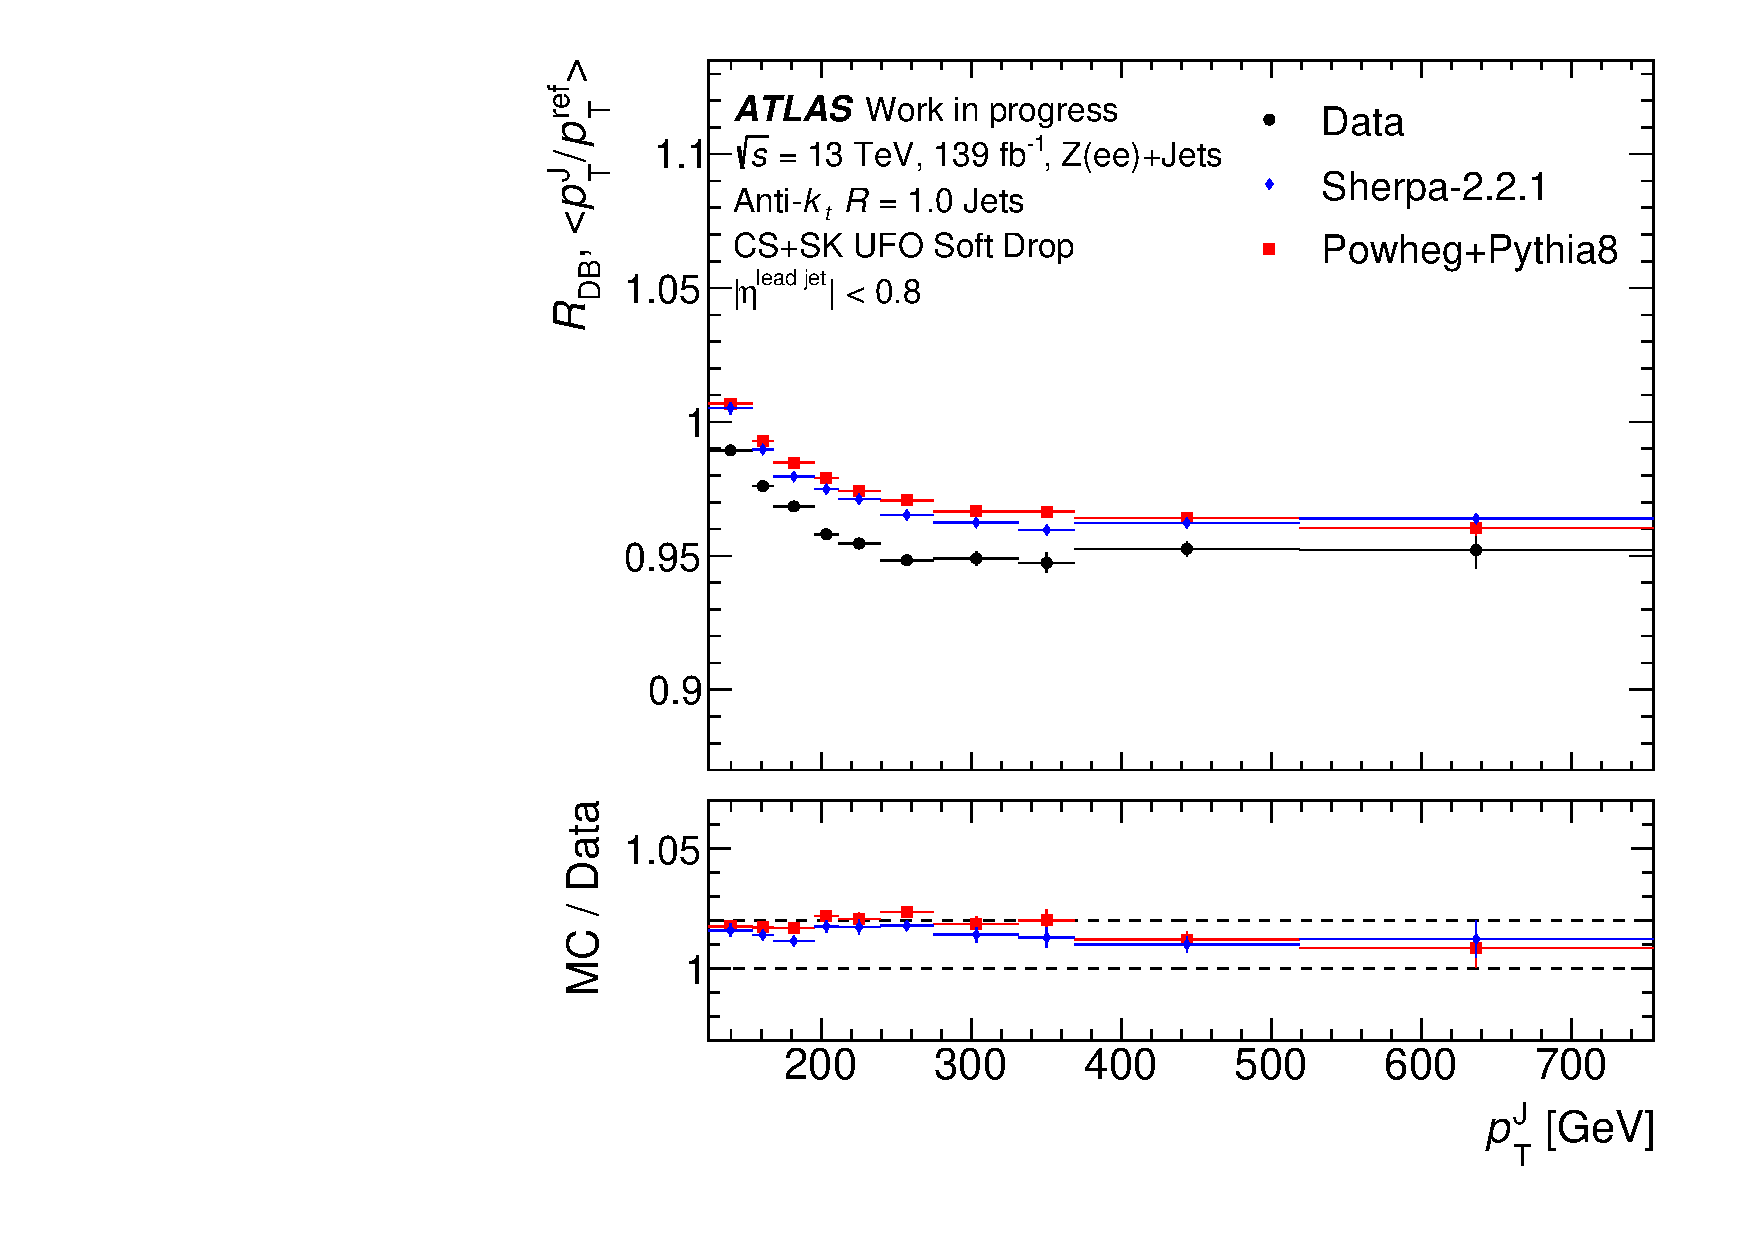
\includegraphics[width=\textwidth]{plots/insitu/Zeejet_response_WIP.pdf}
    \caption{\vspace{20pt}}
    \label{fig:insitufitbal:a}
\end{subfigure}
\hfill
\begin{subfigure}[b]{0.70\textwidth}
    \centering
    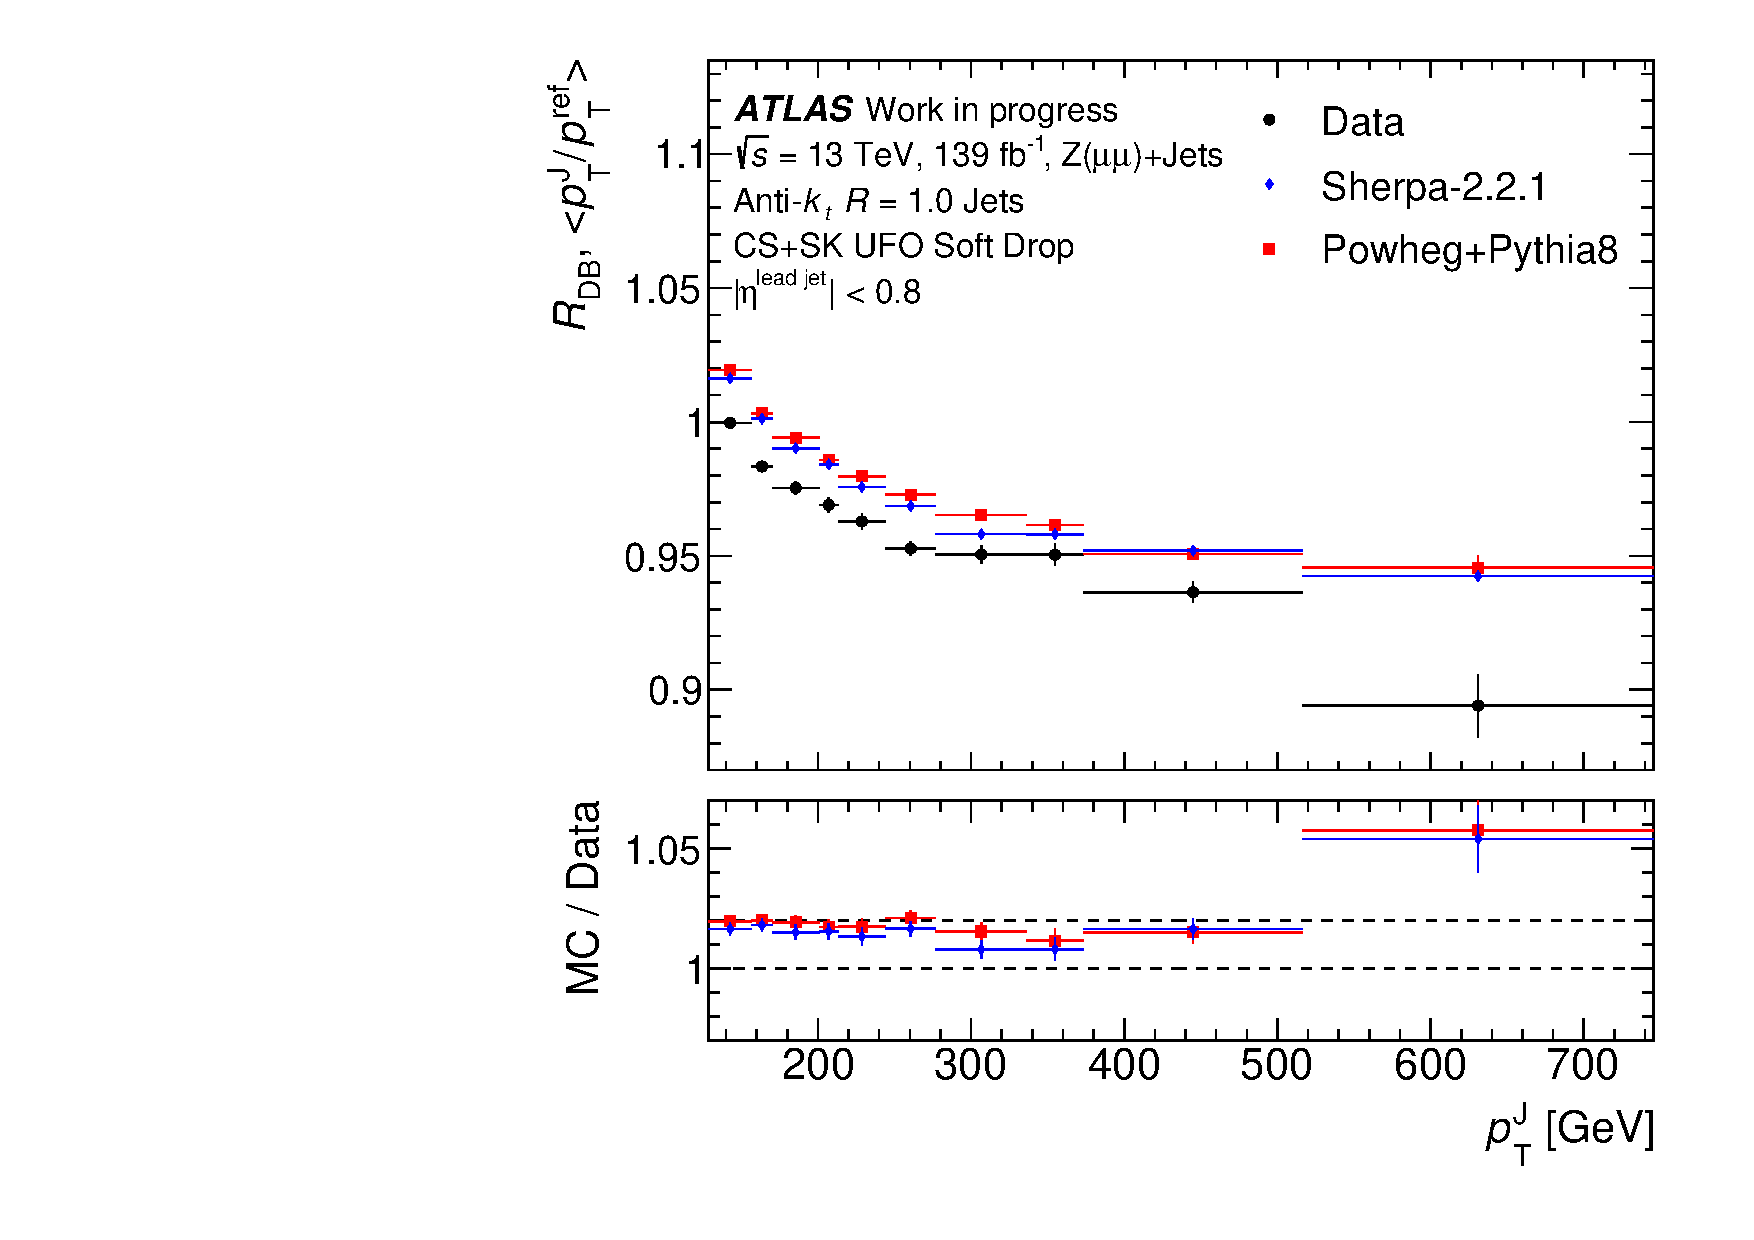
\includegraphics[width=\textwidth]{plots/insitu/Zmmjet_response_WIP.pdf}
    \caption{}
    \label{fig:insitfitbal:b}
\end{subfigure}
\caption{Direct balance response, \rdb, and the double ratio ``MC/Data'' (1/$c$), with leading large-R jet pt \ptJ. The error bars only show statistical uncertainties. (a) shows the response for the electron channel, and (b) shows the muon channel. In the final calibration, the final bin in the muon channel is omitted due to large statistical uncertainty on the response. This comes about because fewer events are selected in the muon channel (also seen in MPF results \cite{Insitu:MPFresults}).\label{fig:nominalfitbalance}}%From MJB documentation: NLO Powheg+Pythia 8 was known to have an issue matching jets with the parton shower, leading to poor modeling of all jet pT, as well as the recoil system pT, as seen in Figure 2 a, c, d.
\end{figure}

\begin{figure}[t]
\centering
\begin{subfigure}[b]{\textwidth}
    \centering
    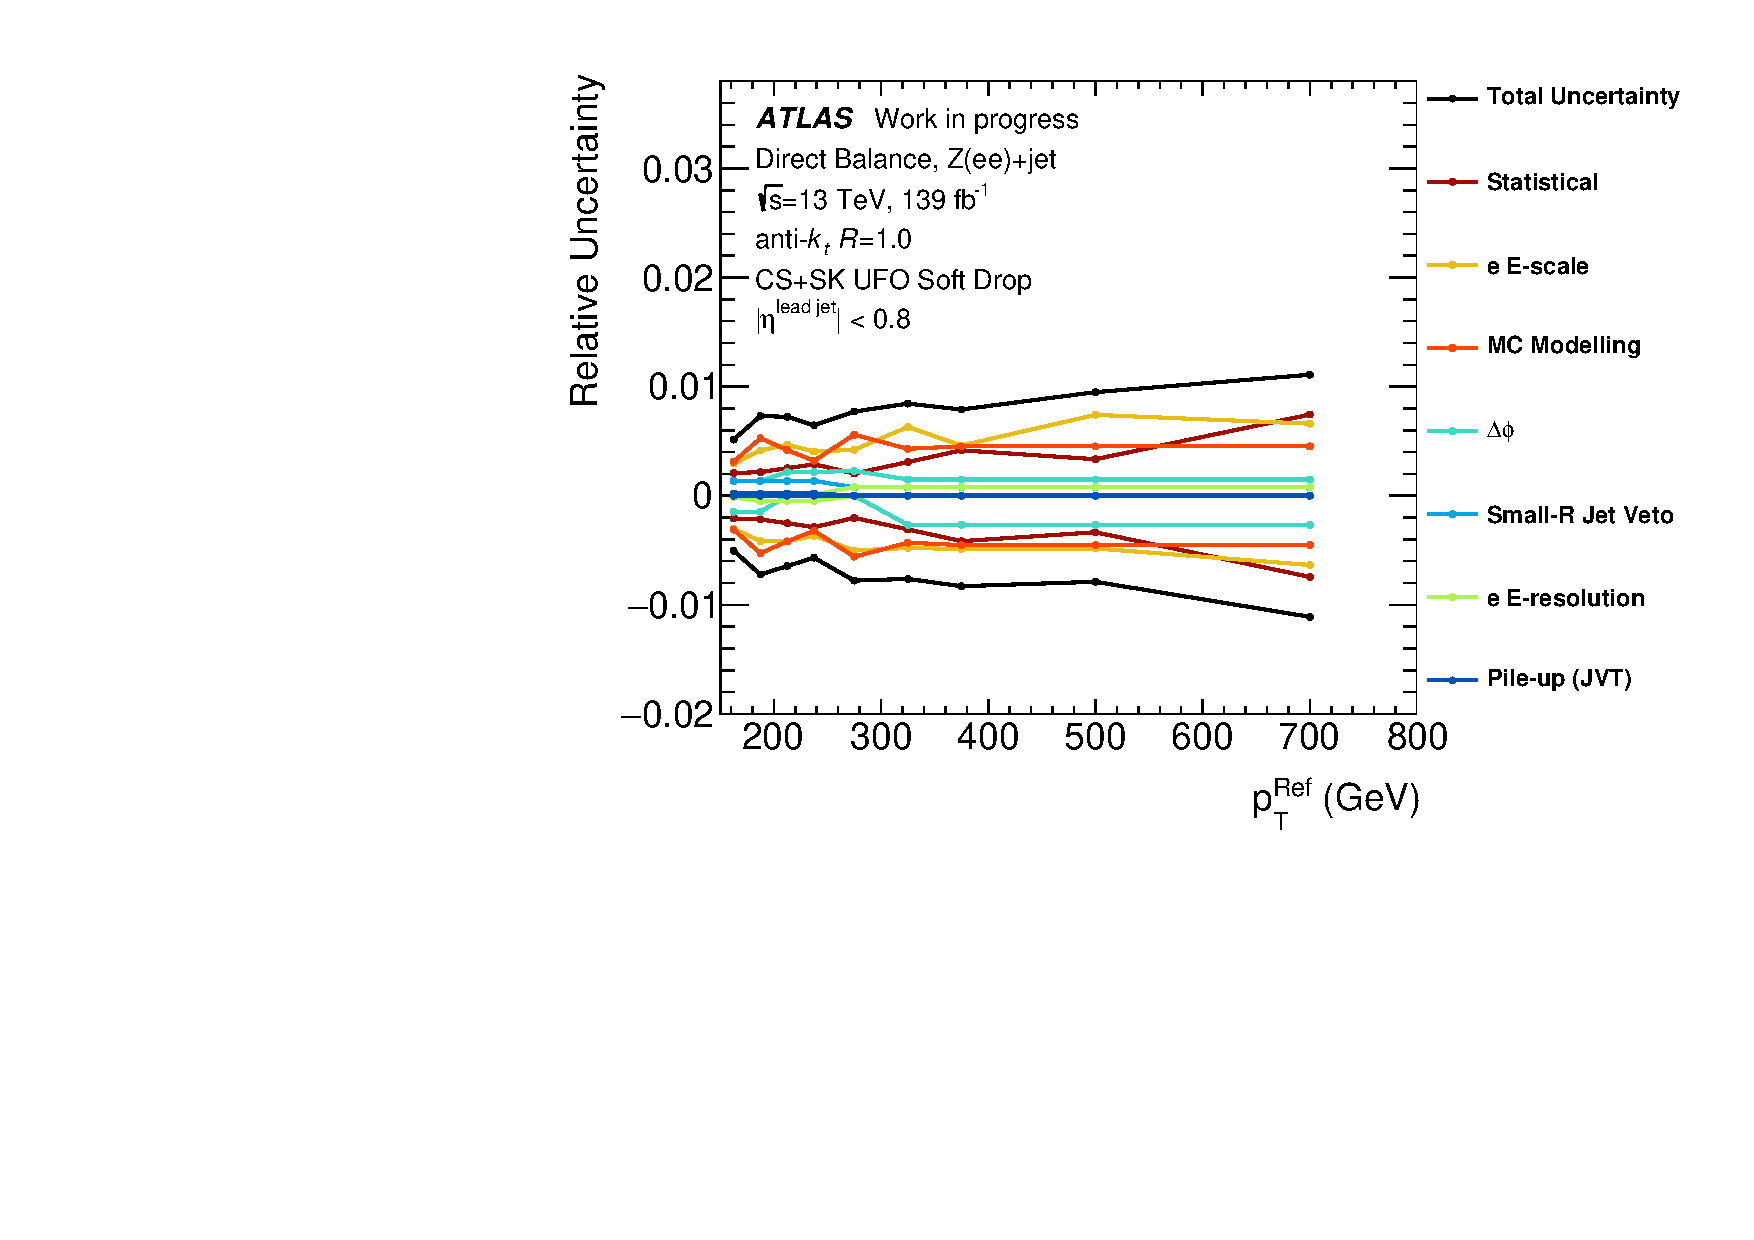
\includegraphics[width=\textwidth]{plots/insitu/unc_ptref_zee_WIP.pdf}
    \caption{\vspace{20pt}}
\end{subfigure}
\hfill
\begin{subfigure}[b]{\textwidth}
    \centering
    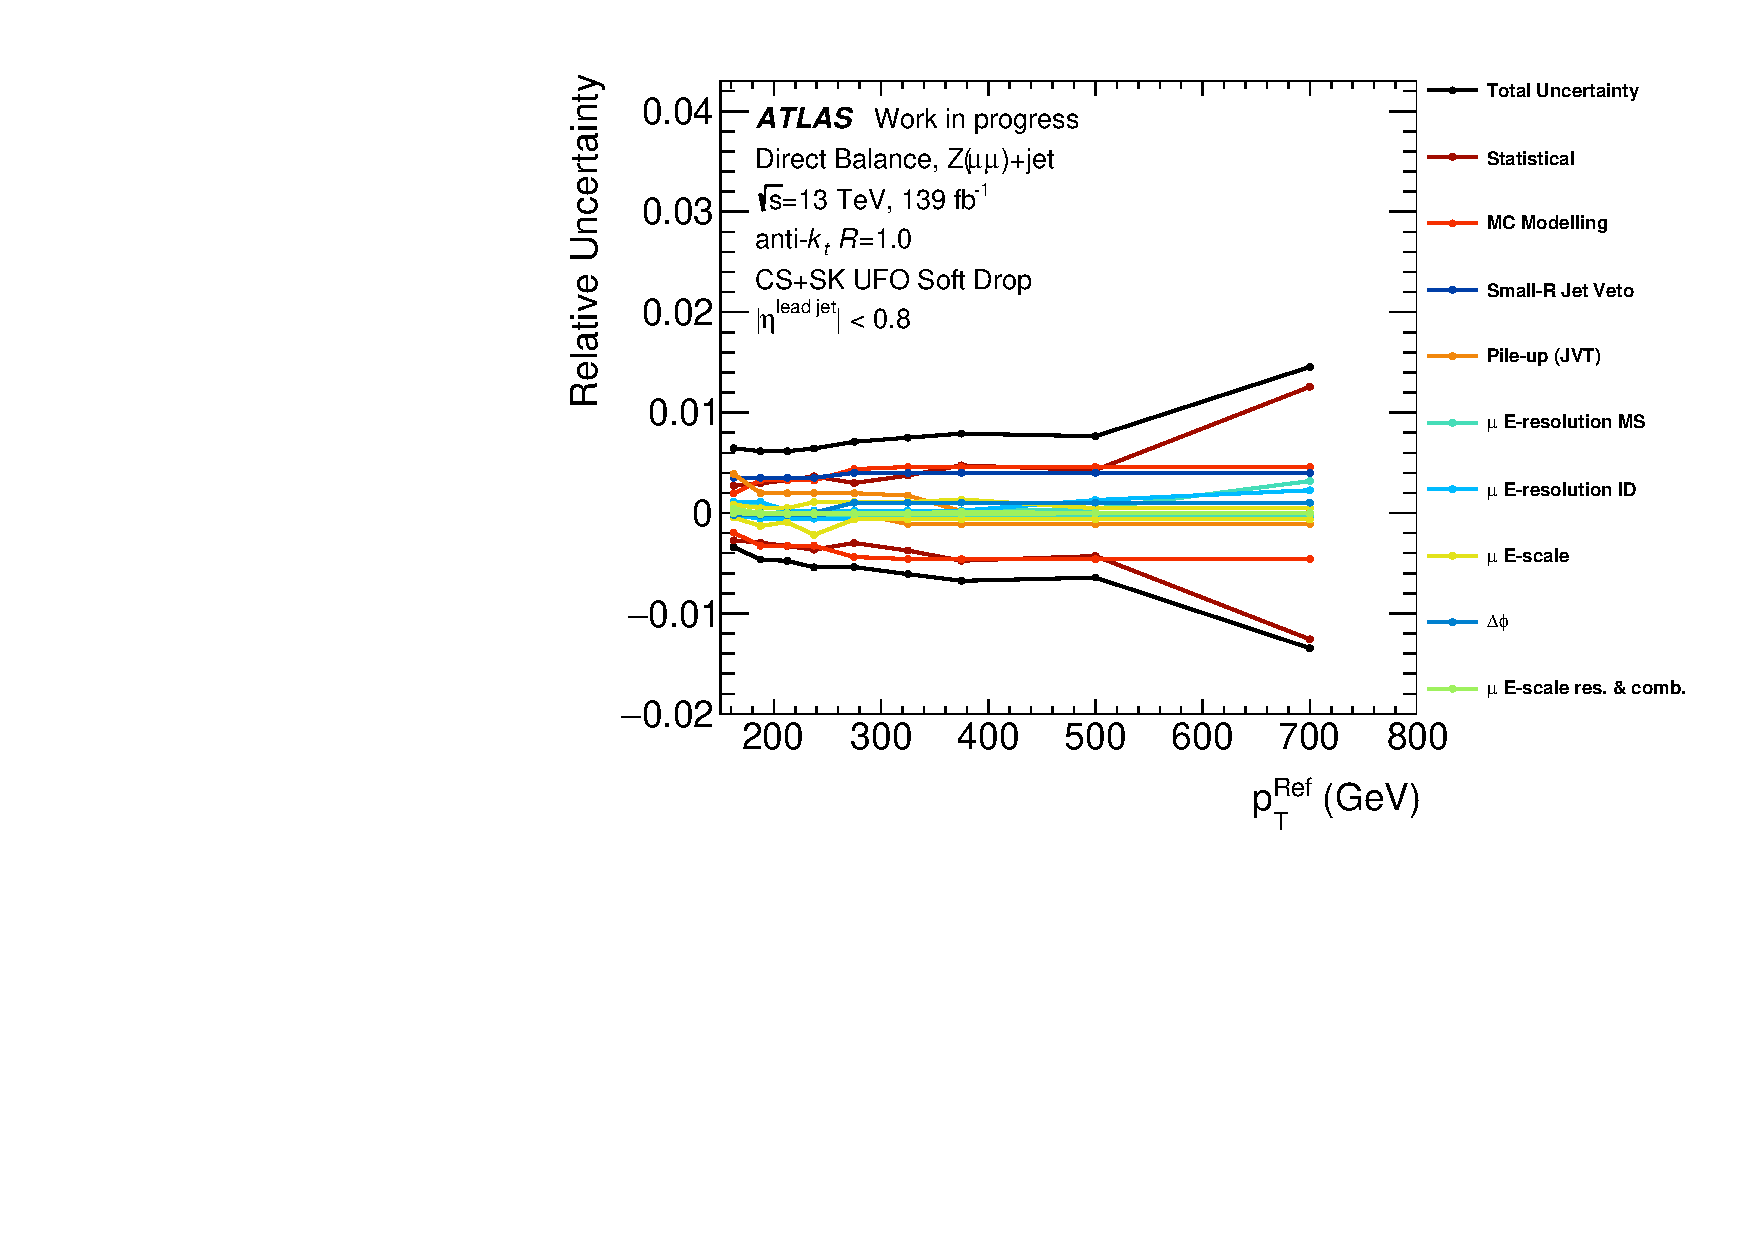
\includegraphics[width=\textwidth]{plots/insitu/unc_ptref_zmm_WIP.pdf}
    \caption{}
\end{subfigure}
\caption{Uncertainties on the double ratio in the electron (a) and muon (b) channels with \ptref before the mapping to \ptJ, and before symmetrising of the uncertainties. For uncertainties which do not have a down variation (for example statistical, MC modelling), a down variation is plotted by simply inverting the sign, this is done only for aesthetic reasons.\label{fig:insitu:ptrefsysts}}
\end{figure}

\begin{figure}[t]
\centering
\begin{subfigure}[b]{\textwidth}
    \centering
    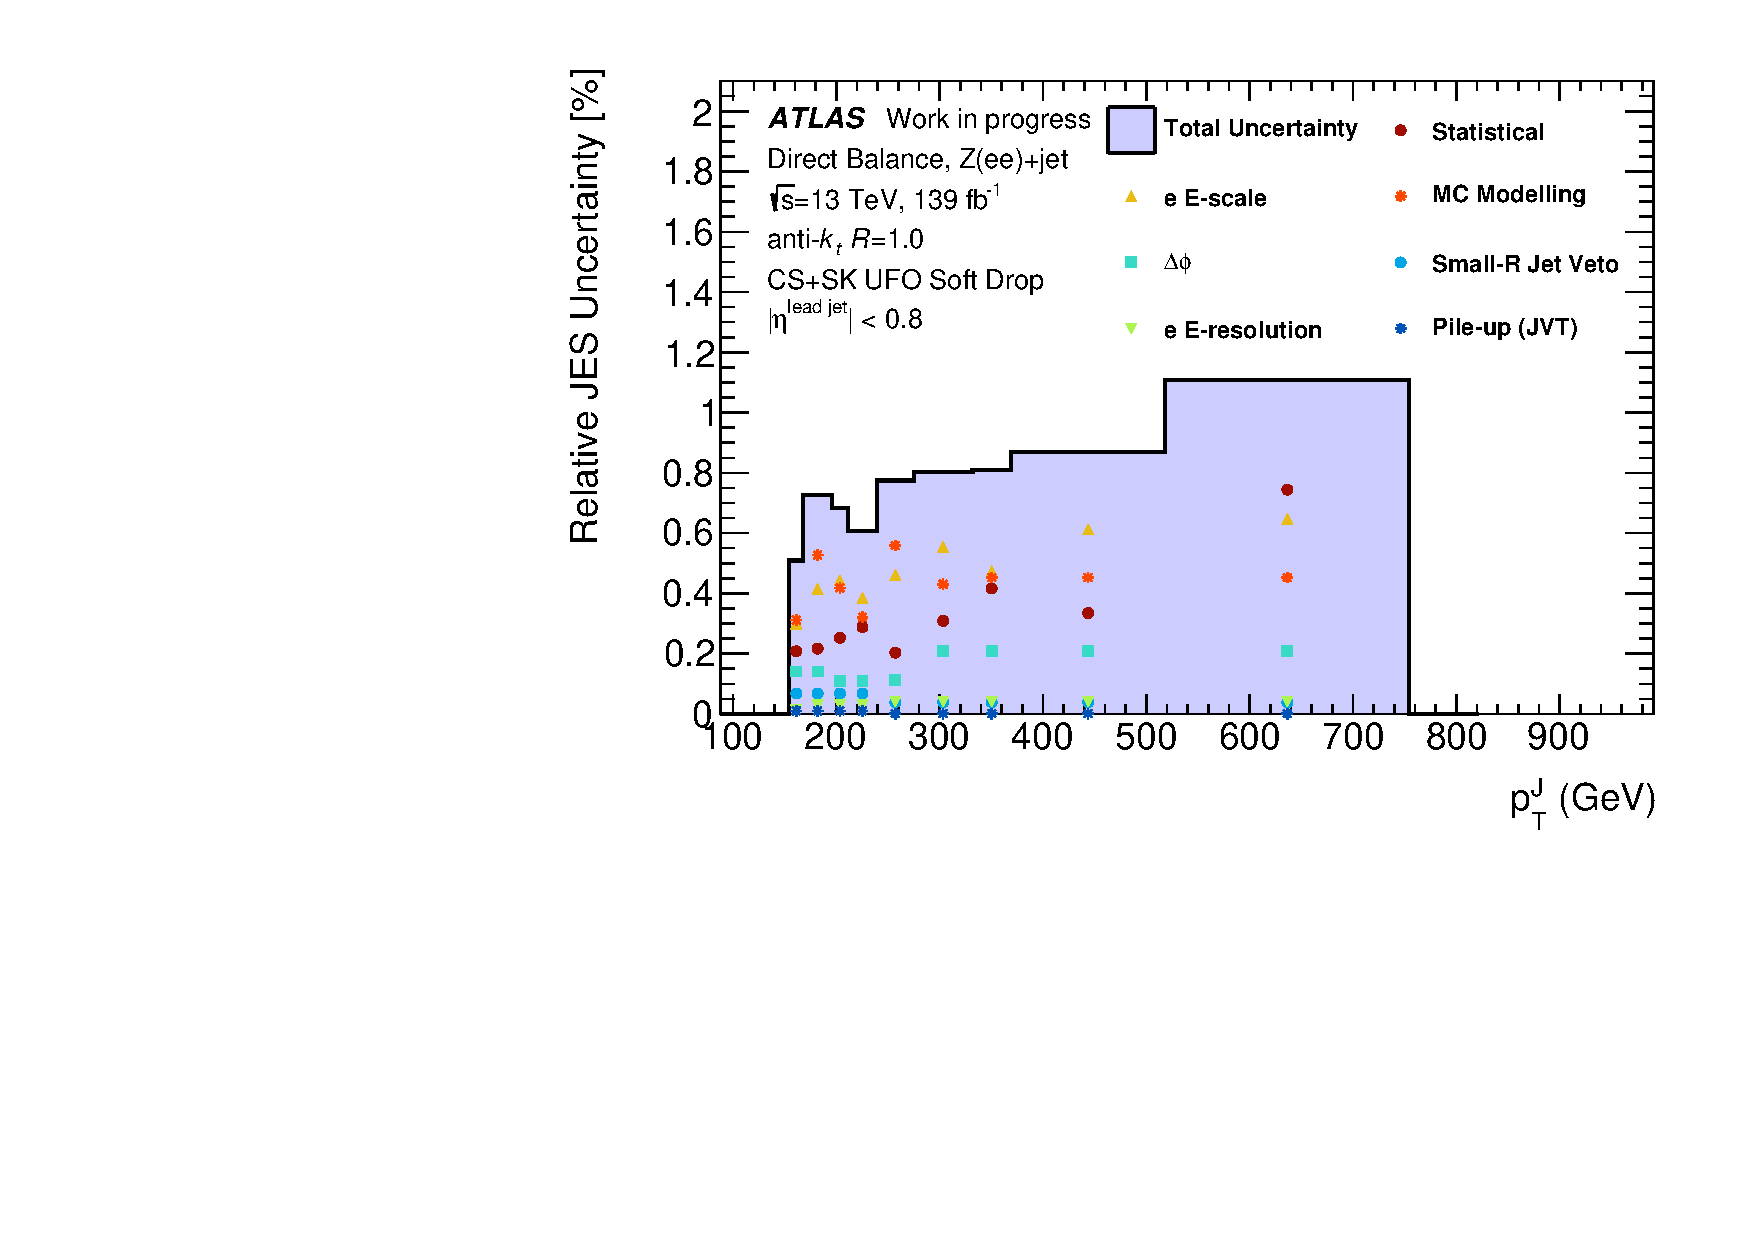
\includegraphics[width=\textwidth]{plots/insitu/systtotal_zee_WIP.pdf}
    \caption{\vspace{20pt}}
\end{subfigure}
\hfill
\begin{subfigure}[b]{\textwidth}
    \centering
    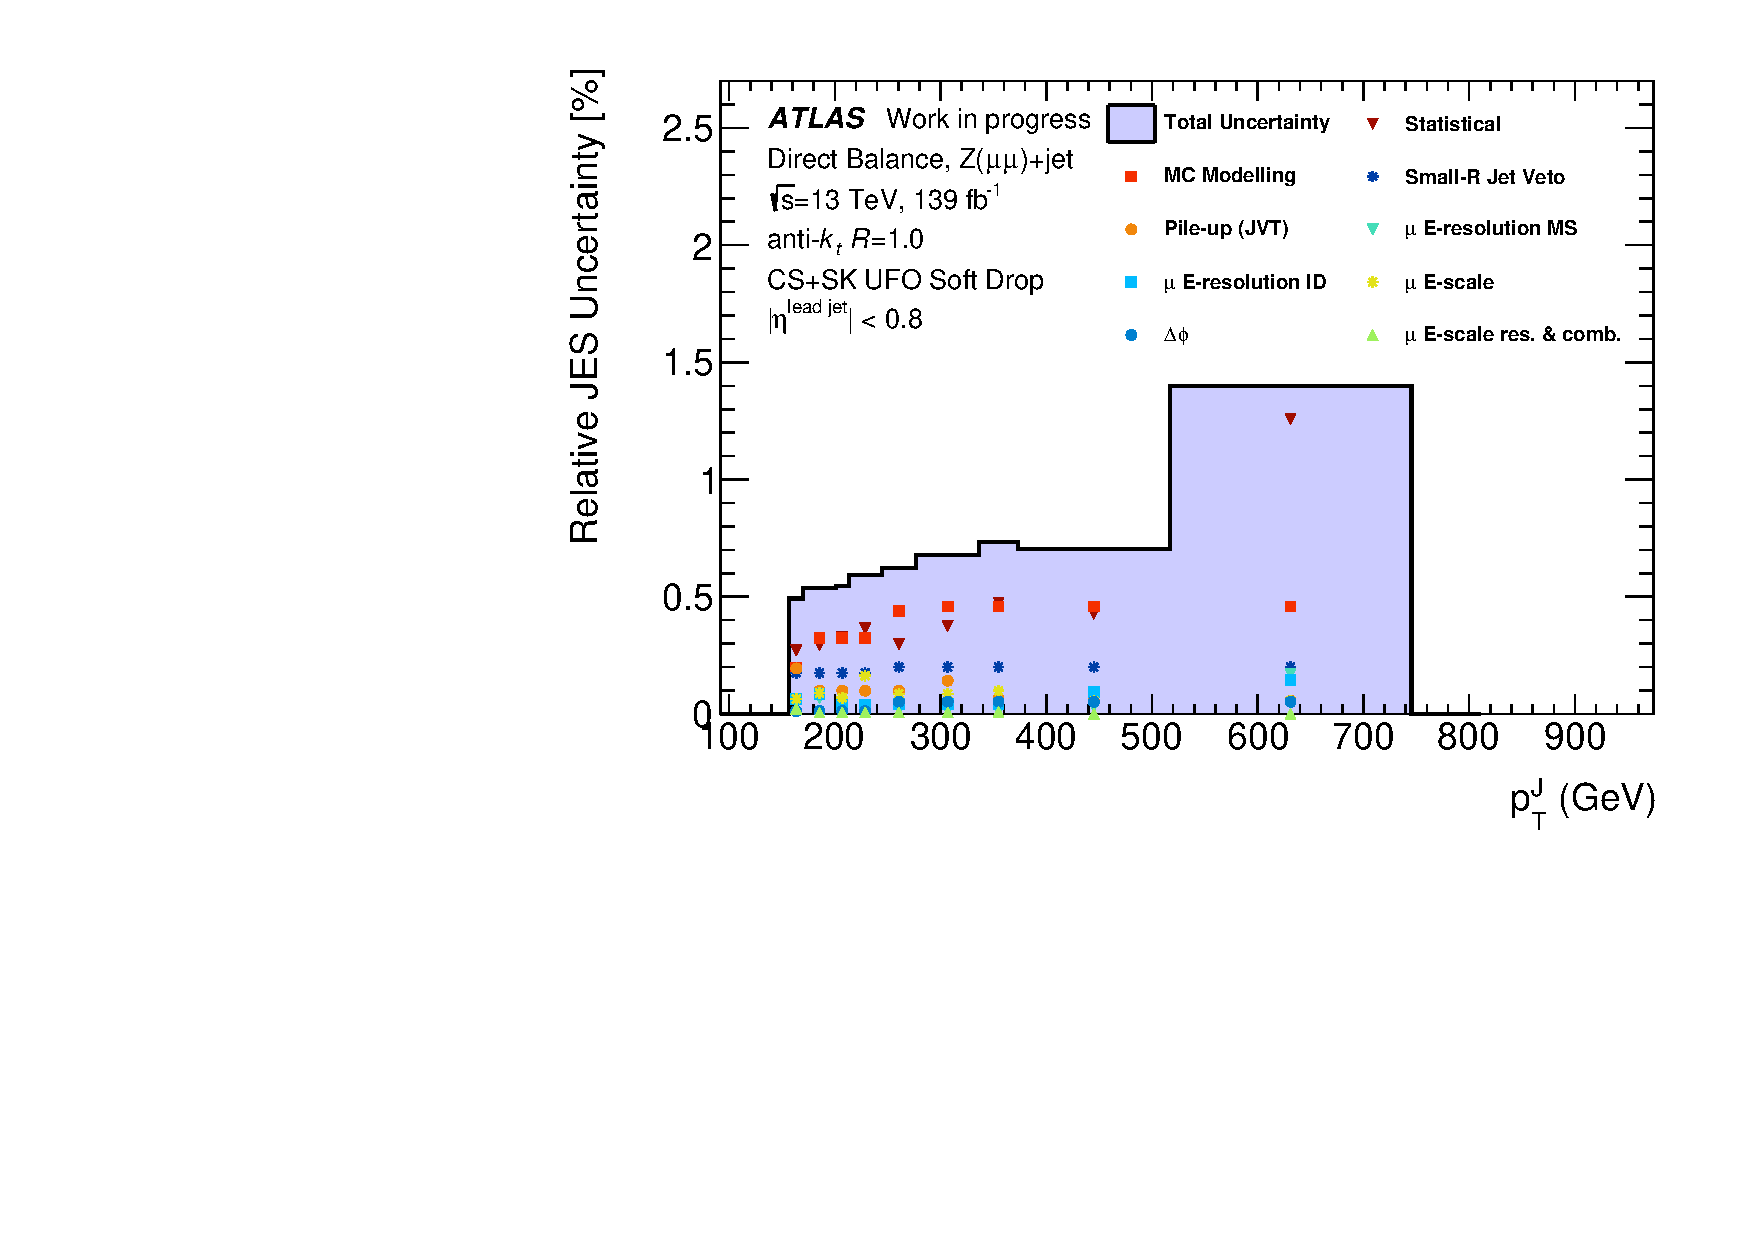
\includegraphics[width=\textwidth]{plots/insitu/systtotal_zmm_WIP.pdf}
    \caption{}
\end{subfigure}
\caption{The final uncertainties on the insitu JES correction with \ptJ and symmetrised uncertainties in the electron (a) and muon (b) channels. Uncertainties are symmetrised by subtracting the down variations from the up variations and dividing by two.\label{fig:insitu:systs}}
\end{figure}

%\clearpage
\section{Insitu combination}

The results in Figures \ref{fig:insitu:systs} and \ref{fig:nominalfitbalance} were used in the insitu combination \cite{Insitu:combination} to derive the precision recommendations for Athena Release-21 large-R UFO jets. In the combination, the $\eta$-intercalibration \cite{Insitu:etainterufo}, $\gamma$+jets \cite{Insitu:gamjetufo}, \zjets \cite{Insitu:zjetufo}, and MJB results \cite{Insitu:mjbufo} are combined to form the final insitu correction factor ($c$) to the JES. The combination of all the $c$ factors and uncertainties is shown in Figure \ref{fig:insitu:combination}. 

\begin{figure}[t]
    \centering
    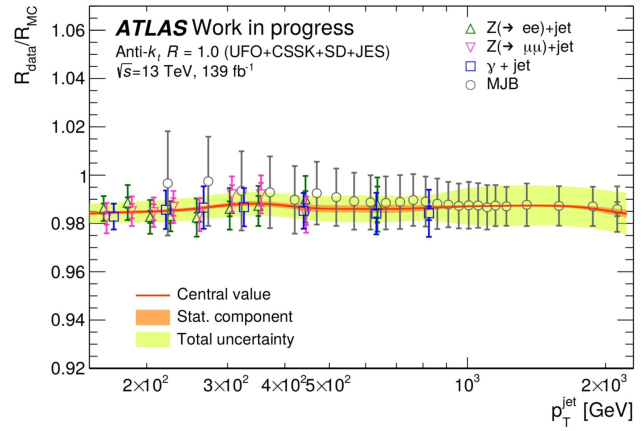
\includegraphics[width=0.8\textwidth]{plots/insitu/combinationplot.pdf}
    \caption{The combination of all the insitu measurements and the final insitu correction factor to the JES, with corresponding statistical and systematic uncertainties. The \zjets and $\gamma+$jets results are in very good agreement. These results are derived completely independently using different software packages. The last data point from the \zmmjets calibration is omitted due to poor statistical precision in this bin. The \zjets and $\gamma$+jets calibrations cover the 150-900\GeV range, and these calibrations typically have $<1\%$ total uncertainty. From around 150-200\GeV the insitu correction is covered solely by \zjets and $\gamma$+jets measurements, and superior precision is seen in the $\gamma$+jets channel. The 150-750\GeV range is covered by all insitu measurements. From around 200-500\GeV, the \zjets channels have the superior precision, and from 500-900\GeV the $\gamma$+jets channel provides the superior measurement. Above 900\GeV, the calibration is solely covered by the MJB measurement. The final uncertainties on the combined calibration are typically below 0.5\%. Figure taken from \cite{Insitu:combination}.\label{fig:insitu:combination}}
\end{figure}

%TODO: Muon large negative weights - mayube
%TODO: Mention bad replicas:    #Ignore obviously bad fits
% if( data_replica <= 0.01 or nominal_means_mc[ireplica] <= 0.01 or data_replica > 4 or nominal_means_mc[ireplica] > 4):
%TODO: Why MC only for CP systematics? Maybe
%TODO: Why muon multiplicity less. Investigate cutflows
%\clearpage
\section{Small-R Insitu Calibration Cross-check}
As an additional cross-check for the small-R EMPflow \zjets insitu calibration, the InsituBalance software framework was used to derive the nominal insitu calibration. This was compared with the nominal insitu calibration derived using the software framework which is usually used for the small-R calibration in ATLAS (the MPF framework). 

\subsection{Samples, object definitions, and event selection}

The comparison was done using 2018 data in the electron channel. Small-R EMPFlow jets are used in the calibration. The 2018 dielectron trigger described in Table \ref{tab:Insitu:trigger} is used. Electrons are required to satisfy ``Loose'' ID and ``Loose'' isolation criteria. Jets are selected in the central $|\eta|<0.8$ region. Jets are calibrated up to the MC JES + GSC (Global Sequential Calibration) level using the 2019 consolidated recommendations. Electrons are calibrated used the same prescription as in Section \ref{sec:insitu:largerobj}. Jets are required to satisfy $\ptj>10\GeV$, and events are selected such that $\Delta\phi(j,Z)>2.8$. In order to reduce contamination from events with large hadronic recoil, a sub-leading jet veto is applied such that $\pt^{\text{second}}<\text{max}(20\GeV,0.1\times\ptref)$, where $\pt^{\text{second}}$ is the \pt of the sub-leading jet. The \textit{Tight} JVT working point is used for jets with $\pt<60\GeV$ and $\eta<2.4$. The only overlap removal requirement is that jets are required to satisfy $\DeltaR(j,Z)>0.2$.

\subsection{Results}

The responses agree very well between the two frameworks, as shown in Figure \ref{fig:insitu:crosscheck}. This serves as a cross-check for the small-R jet calibration, but indeed also gives confidence in the large-R calibration in that the software machinery is behaving as expected.

\begin{figure}[t]
\centering
\begin{subfigure}[b]{\textwidth}
    \centering
    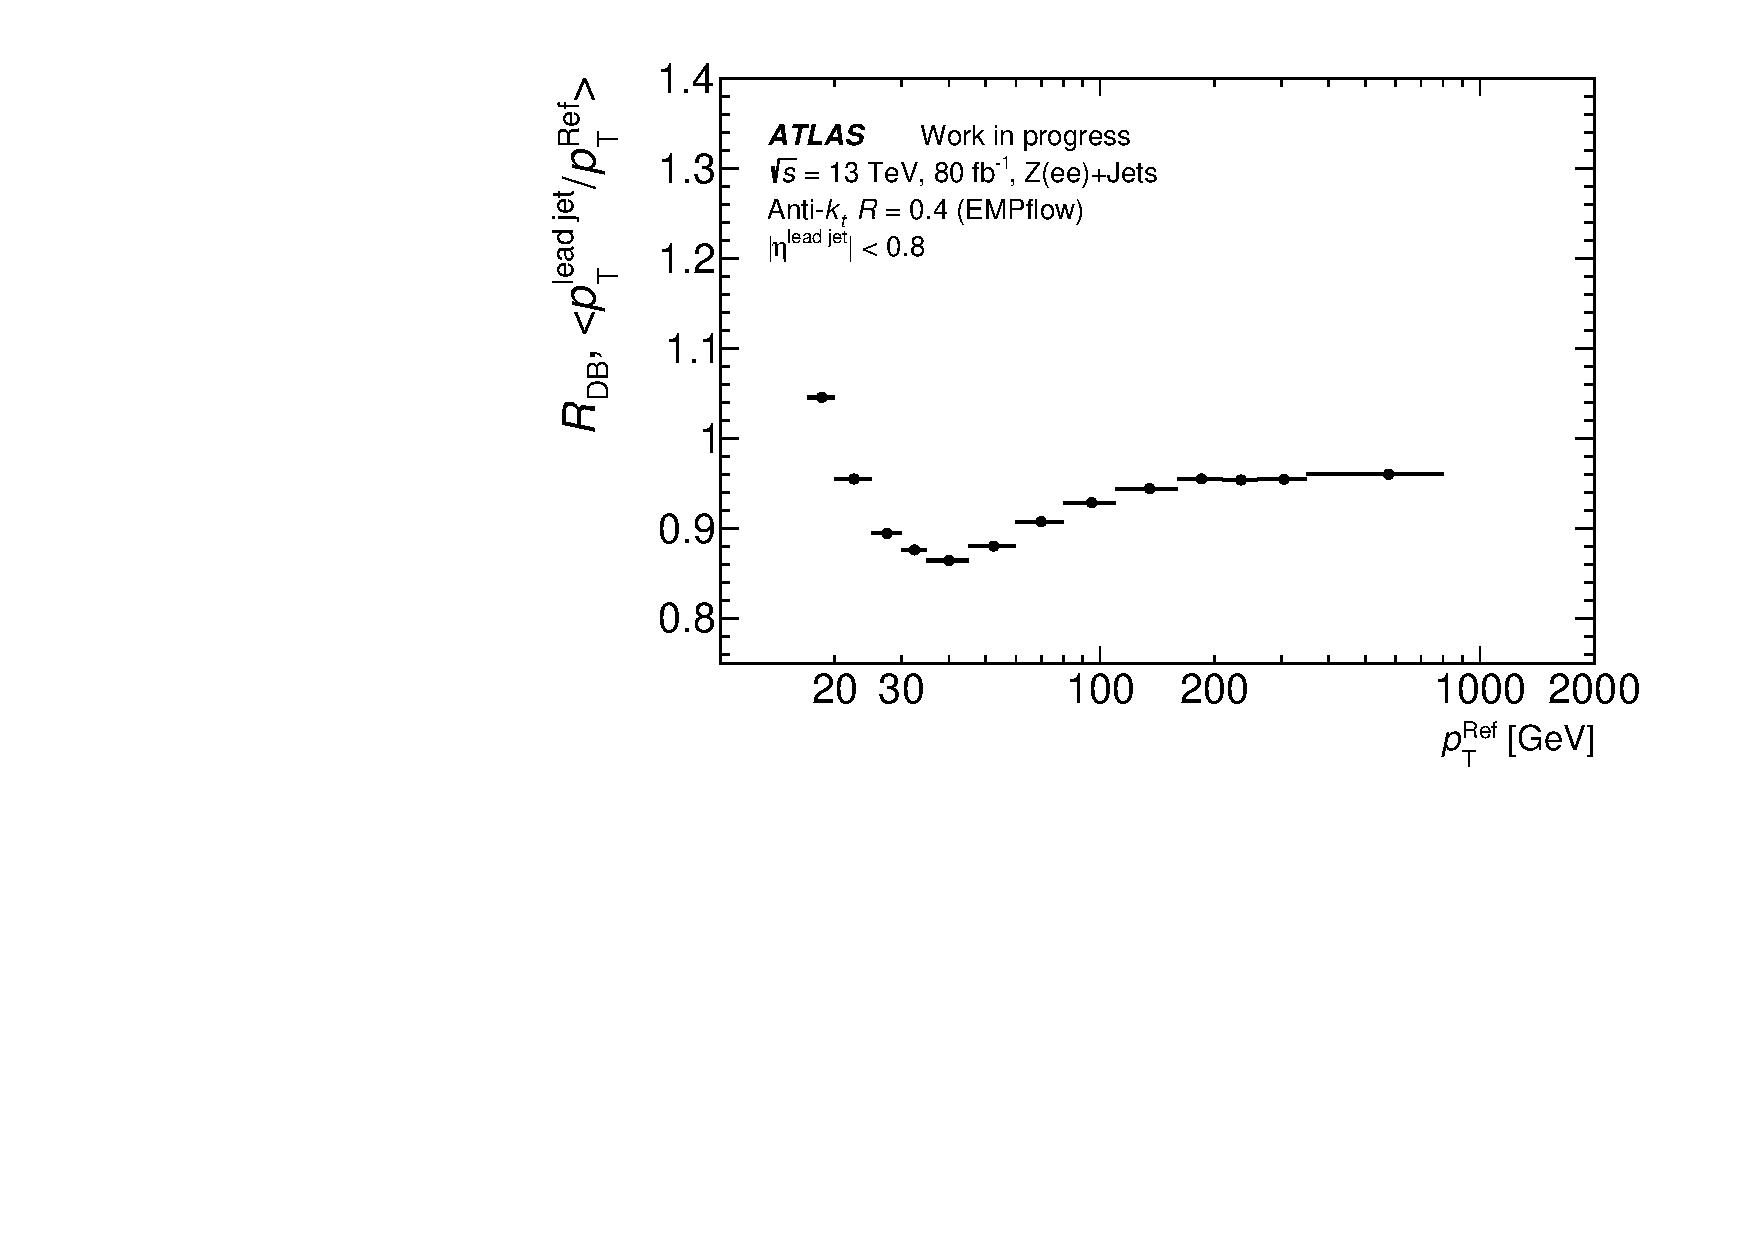
\includegraphics[width=1.05\textwidth]{plots/insitu/SmallRresponse_logX_WIP.pdf}
    \caption{\vspace{20pt}\label{fig:insitu:crosscheck:a}}
\end{subfigure}
\hfill
\begin{subfigure}[b]{\textwidth}
    \centering
    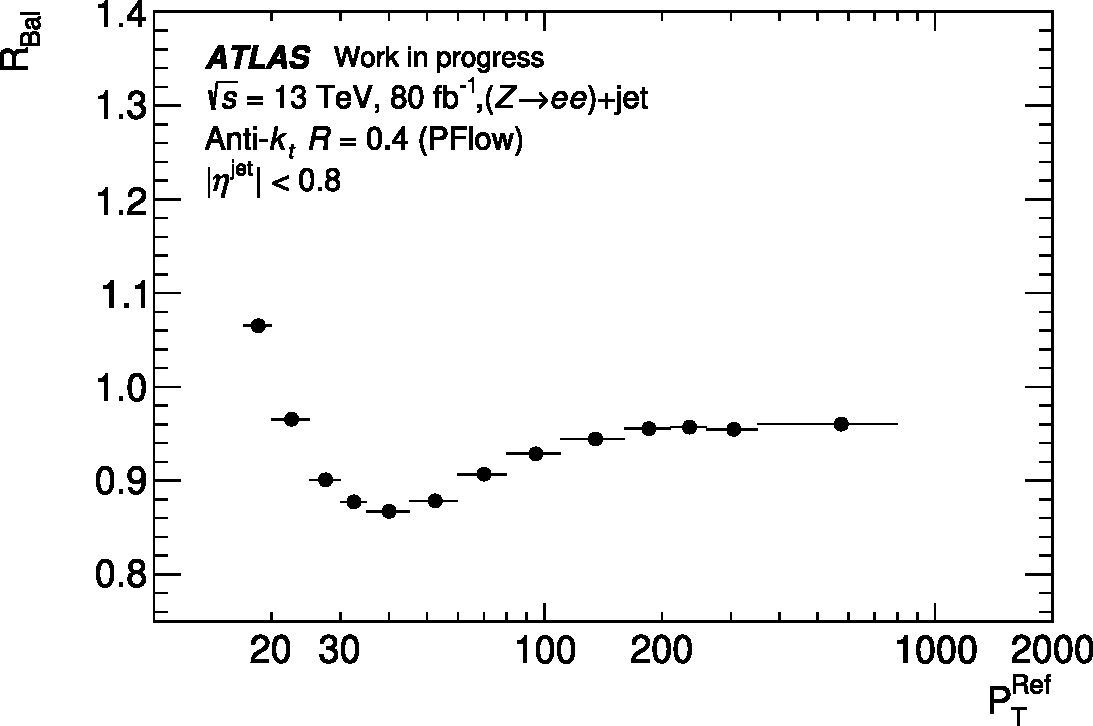
\includegraphics[width=\textwidth]{plots/insitu/MPF_framework_RDB_WIP.pdf}
    \caption{\label{fig:insitu:crosscheck:b}}
\end{subfigure}
\caption{Comparison of the \rdb response between the InsituBalance software framework (a), and the MPF software framework (b) for 2018 data in the electron channel. The slight differences seen when comparing the first low \pt bins can be attributed to slightly different fit functions and fit range in the fits to determine the average response. The MPF framework response plot (b) was produced by Sahil Singh \cite{Insitu:sahilresponse}.\label{fig:insitu:crosscheck}}
\end{figure}

The slight differences between the response in Figures \ref{fig:insitu:crosscheck:a} and \ref{fig:insitu:crosscheck:b} can be attributed to differences in the fit range, fitting function, and binning of \ptbal. The InsituBalance framework uses a Gaussian fit over the fit range given by 1/8 times the maximum bin, and the MPF framework uses a modified Poisson distribution (a continuous generalisation of the Poisson distribution defined using the gamma function) with a dynamic, asymmetric \ptbal range. The was confirmed by explicitly checking the calibrated \ptref and \ptbal values for individual events in the 2018 data sample in the two software frameworks, and equivalent values were obtained. The \ptbal fits in \ptref bins for the InsituBalance framework and MPF framework are shown in Figures \ref{fig:insitu:insitubalancesmallrfits} and \ref{fig:insitu:mpfsmallrfits}, respectively. 

\begin{figure}[t]
    \centering
    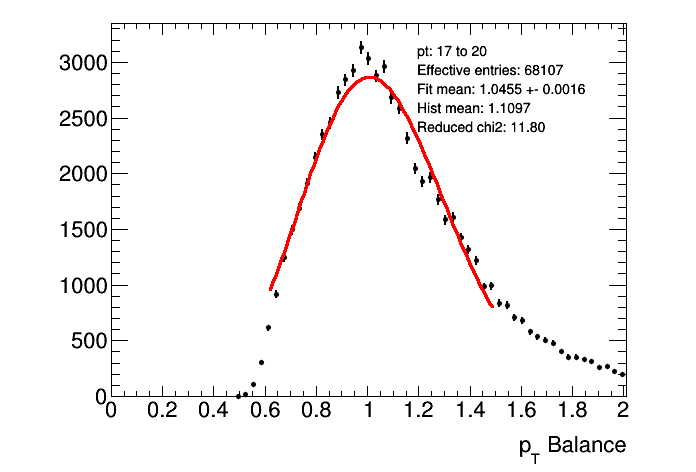
\includegraphics[width=0.31\textwidth]{plots/insitu/fits_insitubalance_smallR/Zeejet_Nominal_Bin0.png}
    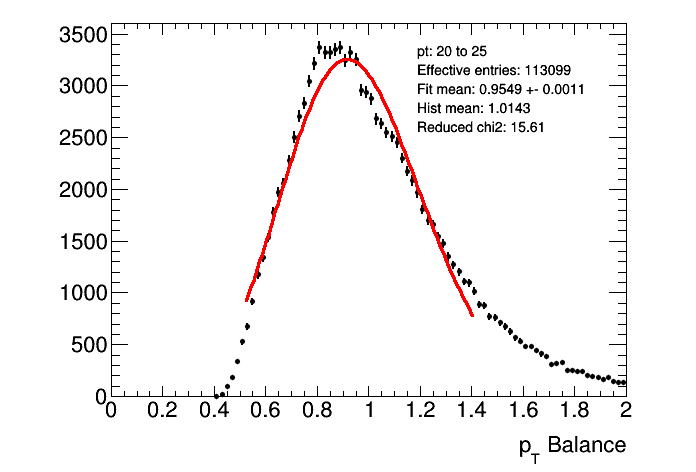
\includegraphics[width=0.31\textwidth]{plots/insitu/fits_insitubalance_smallR/Zeejet_Nominal_Bin1.png}
    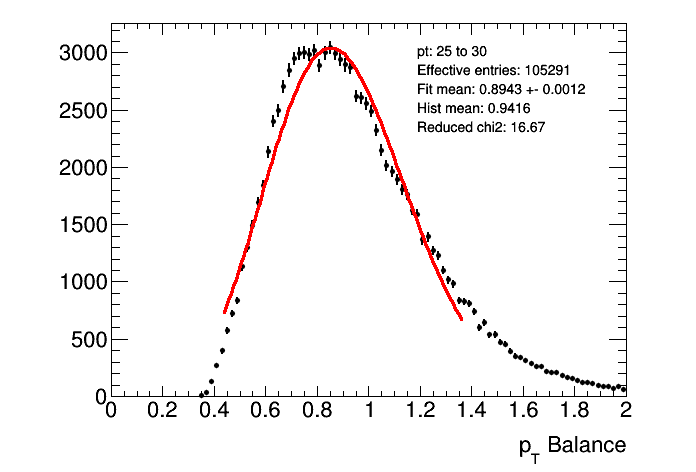
\includegraphics[width=0.31\textwidth]{plots/insitu/fits_insitubalance_smallR/Zeejet_Nominal_Bin2.png}
    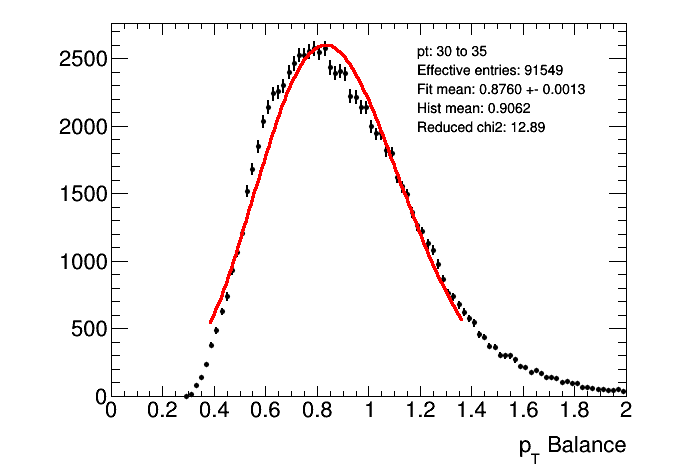
\includegraphics[width=0.31\textwidth]{plots/insitu/fits_insitubalance_smallR/Zeejet_Nominal_Bin3.png}
    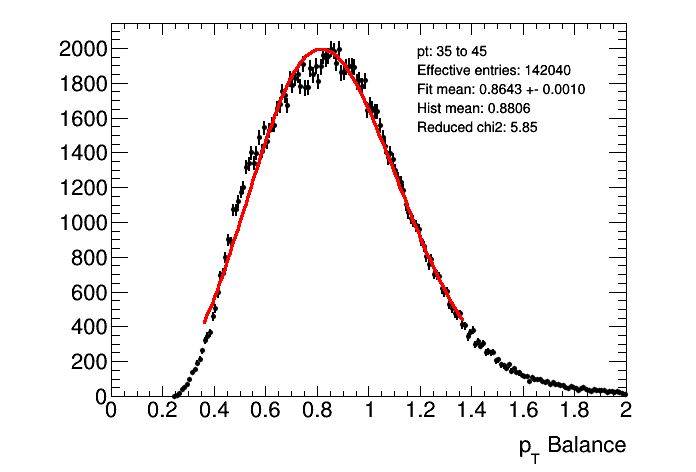
\includegraphics[width=0.31\textwidth]{plots/insitu/fits_insitubalance_smallR/Zeejet_Nominal_Bin4.png}
    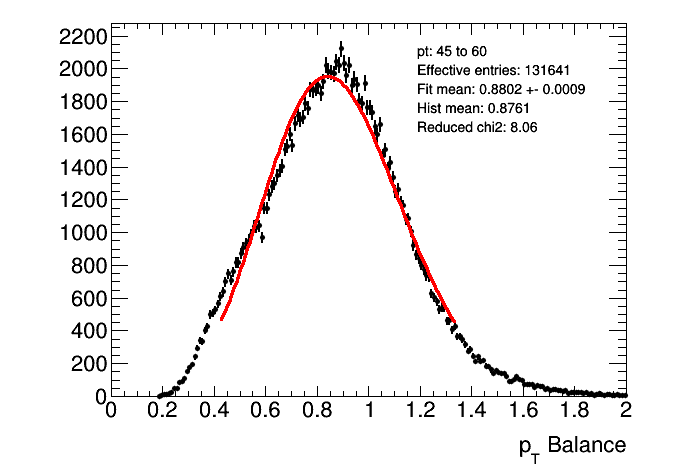
\includegraphics[width=0.31\textwidth]{plots/insitu/fits_insitubalance_smallR/Zeejet_Nominal_Bin5.png}
    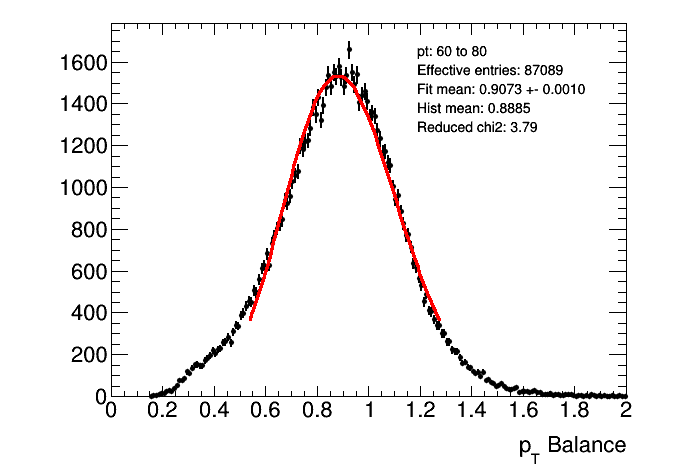
\includegraphics[width=0.31\textwidth]{plots/insitu/fits_insitubalance_smallR/Zeejet_Nominal_Bin6.png}
    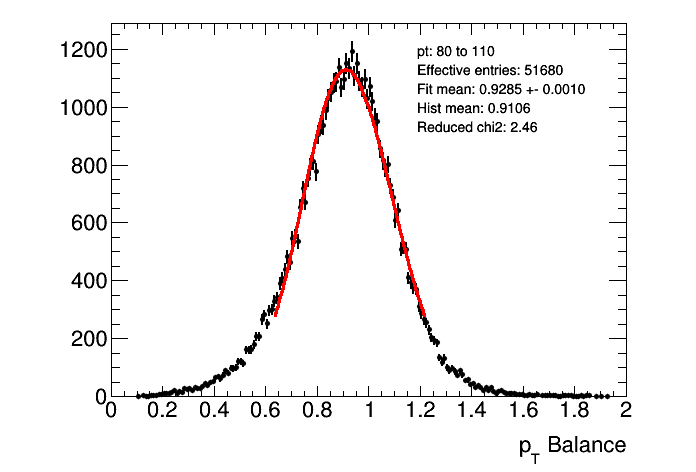
\includegraphics[width=0.31\textwidth]{plots/insitu/fits_insitubalance_smallR/Zeejet_Nominal_Bin7.png}
    \includegraphics[width=0.31\textwidth]{plots/insitu/fits_insitubalance_smallR/Zeejet_Nominal_Bin8.png}
    \includegraphics[width=0.31\textwidth]{plots/insitu/fits_insitubalance_smallR/Zeejet_Nominal_Bin9.png}
    \includegraphics[width=0.31\textwidth]{plots/insitu/fits_insitubalance_smallR/Zeejet_Nominal_Bin10.png}
    \includegraphics[width=0.31\textwidth]{plots/insitu/fits_insitubalance_smallR/Zeejet_Nominal_Bin11.png}
    \includegraphics[width=0.31\textwidth]{plots/insitu/fits_insitubalance_smallR/Zeejet_Nominal_Bin12.png}
    \caption{\ptbal distributions in small-R \zeejets in the InsituBalance software framework. The increase of \rdb at low \ptref can be attributed to the non-Gaussian nature of the low \ptref bins. This behaviour can be attributed to the 10\GeV \ptj cut.\label{fig:insitu:insitubalancesmallrfits}}
\end{figure}

\begin{figure}[t]
    \centering
    \includegraphics[width=0.31\textwidth]{plots/insitu/fits_MPF_smallR/mpf_fit_bin1.pdf}
    \includegraphics[width=0.31\textwidth]{plots/insitu/fits_MPF_smallR/mpf_fit_bin2.pdf}
    \includegraphics[width=0.31\textwidth]{plots/insitu/fits_MPF_smallR/mpf_fit_bin3.pdf}
    \includegraphics[width=0.31\textwidth]{plots/insitu/fits_MPF_smallR/mpf_fit_bin4.pdf}
    \includegraphics[width=0.31\textwidth]{plots/insitu/fits_MPF_smallR/mpf_fit_bin5.pdf}
    \includegraphics[width=0.31\textwidth]{plots/insitu/fits_MPF_smallR/mpf_fit_bin6.pdf}
    \includegraphics[width=0.31\textwidth]{plots/insitu/fits_MPF_smallR/mpf_fit_bin7.pdf}
    \includegraphics[width=0.31\textwidth]{plots/insitu/fits_MPF_smallR/mpf_fit_bin8.pdf}
    \includegraphics[width=0.31\textwidth]{plots/insitu/fits_MPF_smallR/mpf_fit_bin9.pdf}
    \includegraphics[width=0.31\textwidth]{plots/insitu/fits_MPF_smallR/mpf_fit_bin10.pdf}
    \includegraphics[width=0.31\textwidth]{plots/insitu/fits_MPF_smallR/mpf_fit_bin11.pdf}
    \includegraphics[width=0.31\textwidth]{plots/insitu/fits_MPF_smallR/mpf_fit_bin12.pdf}
    \includegraphics[width=0.31\textwidth]{plots/insitu/fits_MPF_smallR/mpf_fit_bin13.pdf}
    \caption{\ptbal distributions in small-R \zeejets in the MPF software framework. A modified Poisson distribution with a dynamic asymmetric fit range is used here.\label{fig:insitu:mpfsmallrfits}}
\end{figure}